%% Journal manuscript placeholder for the extended version of the ECMOR paper.
%% Built from the Elsevier CAS single-column template.

\documentclass[a4paper,fleqn]{cas-sc}

\usepackage[authoryear,longnamesfirst]{natbib}
\usepackage{amsmath,amssymb}
\usepackage{bm}
\usepackage{booktabs}
\usepackage{graphicx}
\usepackage{xcolor}
\usepackage{tikz}
\usetikzlibrary{arrows.meta,calc}
% NOTE: stmaryrd is intentionally NOT loaded. The cas-sc class loads the STIX
% math fonts, which already use all 16 of LaTeX's math symbol-font slots, so
% stmaryrd's \DeclareSymbolFont overflows ("Too many symbol fonts declared").
% STIX provides the same double brackets via \lBrack / \rBrack, used below.

\usepackage{placeins}
\usepackage{float}
\usepackage{capt-of}  % \captionof for non-floating, in-text figures

% Float placement: keep figures near their text and off the end of the paper.
\renewcommand{\topfraction}{0.9}
\renewcommand{\bottomfraction}{0.8}
\renewcommand{\textfraction}{0.07}
\renewcommand{\floatpagefraction}{0.75}

\newcommand{\dd}{\,\mathrm{d}}
\newcommand{\jump}[1]{\lBrack #1 \rBrack}
\newcommand{\Kmat}{\mathbf{K}}
\newcommand{\vflux}{\mathbf{v}}

\newtheorem{theorem}{Theorem}[section]
\newtheorem{lemma}[theorem]{Lemma}
\newtheorem{proposition}[theorem]{Proposition}

\begin{document}
\let\WriteBookmarks\relax
\def\floatpagepagefraction{1}
\def\textpagefraction{.001}

\shorttitle{Locally Conservative CG-LMDFM Flux Reconstruction}
\shortauthors{Harry et al.}

\title[mode=title]{Locally Conservative Flux Reconstruction for Continuous Galerkin Discrete-Fracture Models of Flow and Transport in Fractured Porous Media}

\author[1]{Muchamad Harry Yudha Pratama}
\cormark[1]
\ead{}
\credit{}

\affiliation[1]{organization={Khalifa University of Science and Technology},
            city={Abu Dhabi},
            country={United Arab Emirates}}

\cortext[1]{Corresponding author}

\begin{abstract}
Fractured porous media flow simulation demands accurate fracture--matrix coupling and strict local mass conservation. Lagrange multiplier discrete fracture models (LMDFM) represent fractures as codimension-one interfaces with independent fracture and matrix meshes, enforcing pressure continuity weakly. However, standard continuous Galerkin (CG) discretizations are not locally conservative \citep{Koeppel2019}, limiting their use for conservation-law-based flow models. This work develops locally conservative CG FEM formulations for LMDFM in single-phase Darcy flow. Building on an existing methodology \citep{Koeppel2019}, we propose and compare two distinct strategies to restore local conservation of flux in CG formulations, addressing a key limitation of existing approaches. This framework enables direct comparison between accurate element-wise flux reconstruction and physics-informed learning for restoring local conservation. The first strategy extends an existing flux post-processing method for non-fractured domains \citep{DENG2019166} to the LMDFM setting. Locally conservative fluxes are reconstructed on dual mesh interfaces via independent, element-wise local problems. For a triangular element with Lagrange polynomial space of degree-k, the local problem yields a linear system whose size scales with the number of local degrees of freedom. The local solves are fully decoupled, inexpensive, and parallelizable. Fracture interfaces are included in the local balance, yielding locally conservative matrix and fracture fluxes, exact fracture--matrix exchange, and normal-flux continuity across dual mesh interfaces. The second strategy relies on conservative physics-informed neural networks (cPINNs) to locally correct CG fluxes \citep{Jagtap2020}. Unlike standard PINNs, cPINNs employ domain decomposition and enforce local conservation via continuity of normal fluxes across subdomain interfaces, making them well suited for fractured domains. The networks enforce mass balance in the matrix, fractures, and fracture--matrix interfaces using tailored architectures, adaptive activation functions with trainable slopes to accelerate convergence, and training strategies that keep computational cost comparable to element-wise FEM post-processing. Numerical experiments assess both strategies in terms of computational cost, efficiency, and ease of integration with existing FEM solvers. Convergence tests are presented for matrix and fracture pressures and the Lagrange multiplier across several polynomial degrees, validated against academic tests and benchmark cases, including comparison with the TPFA method implemented in MRST. Finally, we illustrate efficient coupling with a saturation transport equation, present preliminary two-phase flow results, and highlight the potential of the proposed approaches for multiphase flow in fractured porous media.
\end{abstract}

\begin{highlights}
\item Placeholder: fracture-aware locally conservative reconstruction for CG-LMDFM fluxes.
\item Placeholder: deterministic and PINN-based reconstructions compared through multiple conservation diagnostics.
\item Placeholder: journal extensions include higher-order tests, fracture-tip/intersection cases, and expanded transport validation.
\end{highlights}

\begin{keywords}
Fractured porous media \sep Continuous Galerkin finite elements \sep Local conservation \sep Flux reconstruction \sep Lagrange multiplier method \sep Saturation transport
\end{keywords}

\maketitle

\section{Introduction}
\label{sec:introduction}

Natural fractures in subsurface formations create high-permeability flow paths that dominate flow in
hydrocarbon reservoirs, geothermal systems, groundwater aquifers, and subsurface storage sites
\citep{Berkowitz2002, Barenblatt1960, WarrenRoot1963, li2008efficient}. Accurately representing fracture--matrix fluid
exchange is therefore essential in reservoir simulation. Discrete fracture--matrix (DFM) models treat
fractures as lower-dimensional interfaces embedded in the rock matrix, explicitly resolving this exchange
\citep{KarimiFard2004}. Conforming DFM methods align the matrix mesh with fracture faces, which becomes
computationally prohibitive for complex fracture networks. Nonconforming approaches (including immersed finite element methods \citep{zhao2024dfm}, embedded
discrete fracture models (EDFM) \citep{Moinfar2014}, and the Lagrange multiplier discrete fracture model
(LMDFM) of \citet{Koeppel2019}) decouple the fracture and matrix meshes. In the LMDFM, pressure continuity across the fracture is enforced weakly, and
the Lagrange multiplier naturally represents the local fracture--matrix exchange flux.

Continuous Galerkin (CG) finite element methods offer practical advantages for fractured-flow simulation:
they support unstructured meshes, standard variational coupling, and separate finite element spaces for
matrix and fracture unknowns. However, standard CG discretizations
do not produce locally conservative fluxes: the net flux through an element's faces does not, in general,
balance the source term within it \citep{DENG2019166}. This is a fundamental limitation for reservoir
simulation, where transport solvers require an elementwise mass balance to advance saturations and
concentrations. Mixed finite element methods based on Raviart--Thomas spaces \citep{raviart2006mixed, brezzi1991mixed}
provide local conservation by construction but at considerably higher implementation cost. Post-processing
strategies offer a practical alternative to this more complex discretization. \citet{cockburn2007} proposed
a two-step postprocessing for standard CG; \citet{DENG2019166} developed an efficient element-wise
reconstruction on nodal dual control volumes for single-phase flow; and \citet{ZHANG201339} applied a
locally conservative Galerkin approach to two-phase flow in porous media. All three post-processing approaches target non-fractured domains and do not account for the exchange
term that couples the matrix and fracture mass balances. Although \citet{ODSAETER2019edfm} construct a
locally conservative flux for embedded fractured-flow discretizations, their formulation is based on a
single continuous pressure field: the fracture--matrix exchange flux is not an explicit degree of freedom
but is instead recovered implicitly through postprocessing. In the LMDFM, the Lagrange multiplier
$\lambda$ directly approximates this exchange flux, making it a natural ingredient for local balance
correction, a property we exploit in the reconstructions developed below.

Physics-informed neural networks (PINNs) \citep{Raissi2019} offer a mesh-agnostic approach to solving
PDEs by embedding governing equations directly in the training loss. \citet{Jagtap2020} extended this framework to domain-decomposed settings, introducing
conservative PINNs (cPINNs) that enforce zero normal-flux jump across subdomain interfaces.
This makes cPINNs a natural starting point for neural network representations
that must capture fracture-induced flux jumps. \citet{Wang2025} applied improved PINNs to fractured-flow simulation using the reinterpreted
discrete fracture model, but local conservation of the flux was not addressed. To our knowledge, locally conservative flux post-processing for CG-based LMDFM formulations has not been systematically studied.

This paper fills this gap by developing and comparing two post-processing strategies for the CG-LMDFM
flux. The first extends the element-wise reconstruction of \citet{DENG2019166} to the fractured LMDFM
setting by incorporating the Lagrange multiplier exchange in the local balance. The second trains a
physics-informed neural network with a two-network architecture that captures the multiplier-driven flux
discontinuity across the fracture. Three test cases assess local conservation of the reconstructed flux (a nonfractured manufactured
solution, a diagonal crossing-fracture test, and the K\"{o}ppel--Martin boundary-tip benchmark
\citep{Koeppel2019}, including comparison with a MRST/EDFM reference); a fourth couples the reconstructed flux to saturation transport, where replacing the raw CG flux with the PINN-reconstructed flux reduces the global water-balance error from \(18\%\) to \(0.5\%\).
The two strategies are complementary: the numerical reconstruction drives dual-volume residuals to machine
precision, while the PINN approach reduces element-level conservation errors by one to three orders of magnitude;
since it enforces the divergence equation pointwise, this advantage extends beyond element-wise balances
to general control-volume shapes, confirmed by an independent rotated control-volume diagnostic.


\section{Mathematical Model}
\label{sec:model-diagnostics}

We consider a coupled flow and transport problem in a fractured porous medium, in
the hybrid-dimensional setting of the Lagrange-multiplier discrete fracture model
(LMDFM) \citep{Koeppel2019}. The model splits into a pressure problem and a
transport problem for a scalar saturation \(S\), coupled through a
saturation-dependent conductivity. The pressure problem is the total mass
balance---the sum of the phase mass-conservation equations---and sets the total
velocity; the transport problem is the mass-conservation equation of the
transported phase, which advances \(S\). The pressure problem is time-dependent
only through its saturation-dependent coefficient and, in the compressible case,
a storage term, whereas the transport problem carries the genuine time evolution
of the saturation field.
The two are discretized in Section~\ref{sec:flux-reconstruction}, where the
continuous
Galerkin pressure flux is made locally conservative before it drives the
transport.

Let \(\Omega\subset\mathbb{R}^2\) denote the matrix domain and let
\(\Gamma\subset\Omega\) be a lower-dimensional fracture
(Figure~\ref{fig:fracture_schematic}). The matrix pressure is
denoted by \(p\), and the fracture pressure by \(p_\Gamma\). In the Lagrange
multiplier discrete fracture model (LMDFM) \citep{Koeppel2019}, the matrix and
fracture variables may be represented on independent meshes, and pressure
continuity across the fracture is imposed weakly. The multiplier \(\lambda\)
represents the matrix--fracture exchange flux per unit fracture length. It
therefore enters the matrix equation as a concentrated source/sink and the
fracture equation with the opposite sign.

\begin{center}
\centering
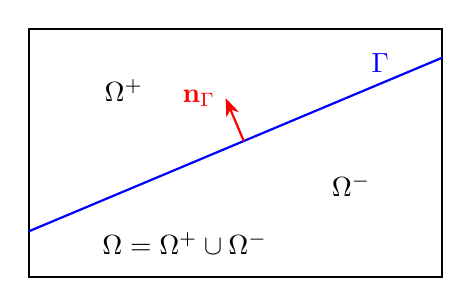
\begin{tikzpicture}[scale=1.05, >=Stealth]
    \draw[thick] (0,0) rectangle (5,3);
    \node at (3,0.15) [anchor=south east] {$\Omega = \Omega^+ \cup \Omega^-$};

    \draw[thick, blue] (0,0.55) -- (5,2.65);
    \node[blue, above] at (4.25,2.35) {$\Gamma$};

    \coordinate (mid) at ($(0,0.55)!0.52!(5,2.65)$);
    \draw[red, ->, thick] (mid) -- ++(-0.22,0.52) node[left] {$\mathbf{n}_\Gamma$};

    \node at (1.15,2.25) {$\Omega^+$};
    \node at (3.9,1.1) {$\Omega^-$};
\end{tikzpicture}
\captionof{figure}{Schematic of a lower-dimensional fracture \(\Gamma\) crossing
the matrix domain \(\Omega\).}
\label{fig:fracture_schematic}
\end{center}

With gravity neglected, the matrix and fracture mass balances, coupled through
\(\lambda\), form the pressure problem, with matrix and fracture
source terms \(f\) and \(f_\Gamma\):
\begin{equation}
\begin{aligned}
c_t\,\partial_t p + \nabla\cdot\left(-\Kmat\nabla p\right) - \lambda \delta_\Gamma &= f
&& \text{in } \Omega,\\
c_{t,\Gamma}\,\partial_t p_\Gamma + \nabla_\Gamma\cdot\left(-\Kmat_\Gamma\nabla_\Gamma p_\Gamma\right) + \lambda &= f_\Gamma
&& \text{on } \Gamma,\\
p|_\Gamma &= p_\Gamma
&& \text{on } \Gamma.
\end{aligned}
\label{eq:lmdfm_strong}
\end{equation}
Here \(\Kmat=\Kmat(S)\) is a saturation-dependent conductivity, a symmetric
positive-definite coefficient that depends on the saturation \(S\) and hence on
time; for brevity we keep the symbol \(\Kmat\) throughout, understanding it to be
evaluated at the current saturation. The coefficient \(c_t\ge 0\) is a storage
coefficient: for \(c_t=0\) the flow is incompressible and the pressure equation is
elliptic at each instant, depending on time only through \(\Kmat(S)\); for \(c_t>0\) the flow is slightly compressible and the pressure
equation is parabolic, carrying its own time derivative. The
saturation enters the pressure problem only through the coefficient \(\Kmat(S)\). When \(c_t=0\) and \(\Kmat\) is
independent of \(S\), the pressure problem decouples and the velocity is frozen.
The fracture conductivity \(\Kmat_\Gamma=\Kmat_\Gamma(S_\Gamma)\) is defined
analogously and includes the fracture aperture, and \(\nabla_\Gamma\) is the
tangential gradient along the fracture. For a straight fracture with unit tangent
\(\bm{\tau}\), \(\nabla_\Gamma p_\Gamma=(\partial_s p_\Gamma)\bm{\tau}\), where
\(s\) is arclength. The term \(\lambda\delta_\Gamma\) denotes a measure
concentrated on the fracture; equivalently,
\[
  \int_\Omega \lambda\delta_\Gamma = \int_\Gamma \lambda .
\]

With \(\vflux=-\Kmat\nabla p\), the multiplier is the jump of the normal Darcy
flux across the fracture \citep{Koeppel2019}. We fix the orientation once and for all: let
\(\Omega^+\) and \(\Omega^-\) denote the two sides of \(\Gamma\), let
\(\mathbf{n}_\Gamma\) be the unit normal pointing from \(\Omega^-\) to
\(\Omega^+\), and for a quantity \(z\) with one-sided traces \(z^\pm\) on
\(\Gamma\) set \(\jump{z}=z^+-z^-\). Explicitly,
\[
  \lambda=\jump{\vflux\cdot\mathbf{n}_\Gamma}
  =-\jump{\Kmat\nabla p\cdot\mathbf{n}_\Gamma}
  \quad \text{on } \Gamma,
\]
that is, writing \(p^+\) and \(p^-\) for the one-sided matrix pressure traces,
\[
  \lambda
  =
  \Kmat\nabla p^-\cdot\mathbf{n}_\Gamma
  -
  \Kmat\nabla p^+\cdot\mathbf{n}_\Gamma .
\]
Thus \(\lambda\) measures the oriented normal-flux imbalance between the two
matrix sides of the fracture.

Let \(V_\Omega\subset H^1(\Omega)\), \(V_\Gamma\subset H^1(\Gamma)\), and
\(\Lambda\subset L^2(\Gamma)\) be the matrix pressure, fracture pressure, and
multiplier spaces. The weak form is: find
\((p,p_\Gamma,\lambda)\in V_\Omega\times V_\Gamma\times\Lambda\) such that, for
all \((q,q_\Gamma,\mu)\in V_\Omega\times V_\Gamma\times\Lambda\),
\begin{equation}
\begin{aligned}
\int_\Omega c_t\,\partial_t p\,q
+\int_\Gamma c_{t,\Gamma}\,\partial_t p_\Gamma\,q_\Gamma
+\int_\Omega \Kmat\nabla p\cdot\nabla q
+\int_\Gamma \Kmat_\Gamma\nabla_\Gamma p_\Gamma\cdot\nabla_\Gamma q_\Gamma
-\int_\Gamma \lambda\left(q|_\Gamma-q_\Gamma\right)
&=
\int_\Omega f q
+\int_\Gamma f_\Gamma q_\Gamma,\\
\int_\Gamma \mu\left(p|_\Gamma-p_\Gamma\right)&=0.
\end{aligned}
\label{eq:lmdfm_weak}
\end{equation}
The first equation is the coupled matrix--fracture mass balance, and the second
enforces pressure continuity across \(\Gamma\) through the multiplier test
functions.

The saturation is advanced by a transport equation in fractional-flow form: the
transported-phase flux is the fractional flow \(F(S)\) times the total velocity
\(\vflux\) \citep{Lie2019}. We assume the fluids are only
slightly compressible, so the compressible accumulation \(c_t\,S\,\partial_t p\)
in the phase balance is small relative to the porosity term \(\phi\,\partial_t S\)
and is neglected; the storage is retained only in the pressure problem (the
\(c_t\,\partial_t p\) and \(c_{t,\Gamma}\,\partial_t p_\Gamma\) terms), where it
keeps the pressure unsteady and sets the time-dependent total velocity that drives
the transport. With porosity \(\phi\) and a source/sink \(q\), the matrix
saturation then satisfies
\begin{equation}
  \phi\,\partial_t S
  + \nabla\cdot\!\left(F(S)\,\vflux\right)
  = q - Q_{m\to\Gamma}
  \quad\text{in }\Omega ,
\label{eq:transport_matrix}
\end{equation}
and the fracture saturation satisfies the one-dimensional analogue
\begin{equation}
  \phi_\Gamma\,\partial_t S_\Gamma
  + \partial_s\!\left(F(S_\Gamma)\,\vflux_\Gamma\cdot\bm\tau\right)
  = q_\Gamma + Q_{m\to\Gamma}
  \quad\text{on }\Gamma ,
\label{eq:transport_fracture}
\end{equation}
where \(\phi_\Gamma\) is the fracture porosity,
\(\vflux_\Gamma=-\Kmat_\Gamma\nabla_\Gamma p_\Gamma\) is the fracture total
velocity, \(s\) is arclength, and \(q_\Gamma\) is the fracture source/sink. The
matrix--fracture exchange of the transported
scalar is the corresponding fraction of the total exchange carried by the
multiplier,
\[
  Q_{m\to\Gamma} = F(S_{\mathrm{up}})\,\lambda ,
\]
with \(S_{\mathrm{up}}\) upwinded according to the sign of the oriented total
exchange \(\lambda\). The system is closed with an initial condition
\(S(\cdot,0)=S_0\) and an inflow condition prescribing \(S\) on the inflow part of
the boundary.

Because the conductivity \(\Kmat(S)\) enters the pressure problem and the total
velocity \(\vflux\) enters the transport problem, the two are coupled both ways:
as the saturation field advances, \(\Kmat(S)\) changes, the pressure field is
updated, and the new velocity advects the saturation further. This coupling is
resolved by the sequential time-stepping algorithm of
Section~\ref{sec:flux-reconstruction}, in which the locally conservative
reconstructed flux drives the transport.

\section{Discretization}
\label{sec:flux-reconstruction}

This section discretizes the model of Section~\ref{sec:model-diagnostics}. The
pressure problem is solved by a continuous Galerkin (CG) LMDFM method, the
transport problem by a standard finite-volume (FV) scheme, and the two are
advanced sequentially in time. Because the CG pressure flux is not locally
conservative, it is post-processed into a conservative flux---by a numerical local
reconstruction (Section~\ref{subsec:nlr}) or a learning-based one
(Section~\ref{subsec:pinn-reconstruction})---before it drives the transport.

We begin with the pressure solve. The continuous Galerkin discretization is
obtained by replacing the continuous
spaces with finite element spaces \(V_{\Omega,h}\), \(V_{\Gamma,h}\), and
\(\Lambda_h\). We seek
\((p_h,p_{\Gamma,h},\lambda_h)\in V_{\Omega,h}\times V_{\Gamma,h}\times
\Lambda_h\) such that, for all
\((q_h,q_{\Gamma,h},\mu_h)\in V_{\Omega,h}\times V_{\Gamma,h}\times\Lambda_h\),
\begin{equation}
\begin{aligned}
\int_\Omega \Kmat\nabla p_h\cdot\nabla q_h
+\int_\Gamma \Kmat_\Gamma\nabla_\Gamma p_{\Gamma,h}\cdot\nabla_\Gamma q_{\Gamma,h}
-\int_\Gamma \lambda_h\left(q_h|_\Gamma-q_{\Gamma,h}\right)
&=
\int_\Omega f q_h
+\int_\Gamma f_\Gamma q_{\Gamma,h},\\
\int_\Gamma \mu_h\left(p_h|_\Gamma-p_{\Gamma,h}\right)&=0.
\end{aligned}
\label{eq:lmdfm_cg}
\end{equation}

Equation~\eqref{eq:lmdfm_cg} is the compact incompressible pressure system,
corresponding to \(c_t=c_{t,\Gamma}=0\) in \eqref{eq:lmdfm_weak}. If
compressible flow is considered, the same CG-LMDFM discretization is used after
adding the storage terms
\(\int_\Omega c_t\,\partial_t p_h\,q_h\) and
\(\int_\Gamma c_{t,\Gamma}\,\partial_t p_{\Gamma,h}\,q_{\Gamma,h}\) to the
left-hand side. With backward Euler at \(t^{n+1}\), these become the mass terms
\((c_t/\Delta t)\int_\Omega p_h^{n+1}\,q_h\) and
\((c_{t,\Gamma}/\Delta t)\int_\Gamma p_{\Gamma,h}^{n+1}\,q_{\Gamma,h}\), with the
previous-time-level contributions moved to the right-hand side.

Because the multiplier \(\lambda_h\) ties the fracture and matrix
pressures together, \eqref{eq:lmdfm_cg} is a saddle-point system whose stability
requires a discrete inf--sup (LBB) condition between the multiplier space
\(\Lambda_h\) and the pressure traces on \(\Gamma\). \citet{Koeppel2019} establish
this condition for the present formulation: it holds when the multiplier mesh
(size \(h_\lambda\)) is kept coarse relative to the matrix mesh (size \(h\)). For a piecewise-constant
multiplier the scheme is stable and convergent provided \(h_\lambda\gtrsim 3h\)
(their Hypothesis~1 and Remark~1), whereas for a continuous piecewise-linear
multiplier a unique solution exists but convergence is not guaranteed; we
therefore keep the multiplier mesh coarse on the nonconforming meshes below.

% Because the multiplier \(\lambda_h\) enters \eqref{eq:lmdfm_cg} as a constraint
% that ties the fracture and matrix pressures together, the system is of
% saddle-point type, and its stability hinges on the multiplier--pressure coupling
% term already present in \eqref{eq:lmdfm_cg},
% \begin{equation}
%   b\big((q_h,q_{\Gamma,h}),\mu_h\big)
%   =\int_\Gamma \mu_h\,(q_h|_\Gamma-q_{\Gamma,h}),
%   \label{eq:bform}
% \end{equation}
% which measures how strongly a trial multiplier \(\mu_h\) acts on the pressure jump
% \(q_h|_\Gamma-q_{\Gamma,h}\) across the fracture. Such a system is well posed only
% when every multiplier is genuinely felt by some pressure pair---the discrete
% inf--sup (or LBB) condition \citep{brezzi1991mixed}: there is a constant
% \(\beta>0\), independent of the mesh, such that
% \begin{equation}
%   \inf_{0\neq\mu_h\in\Lambda_h}\;
%   \sup_{0\neq(q_h,q_{\Gamma,h})\in V_{\Omega,h}\times V_{\Gamma,h}}
%   \frac{b\big((q_h,q_{\Gamma,h}),\mu_h\big)}
%        {\|(q_h,q_{\Gamma,h})\|_{V}\,\|\mu_h\|_{\Lambda}}
%   \;\ge\;\beta,
%   \label{eq:infsup}
% \end{equation}
% with the pressure energy norm
% \(\|(q_h,q_{\Gamma,h})\|_V^2=\int_\Omega|\nabla q_h|^2+\int_\Gamma|\nabla_\Gamma q_{\Gamma,h}|^2\)
% and the mesh-weighted multiplier norm
% \(\|\mu_h\|_\Lambda=h_\lambda^{1/2}\,\|\mu_h\|_{L^2(\Gamma)}\) (the discrete
% \(H^{-1/2}\) norm of \citealp{Koeppel2019}, their Eq.~(20)). In words,
% \eqref{eq:infsup} says that no matter which multiplier one picks, some pressure
% pair responds to it by at least a fixed amount \(\beta\) that does not deteriorate
% as the mesh is refined. This fails when the multiplier space is too rich---its
% mesh too fine relative to the matrix mesh---so that some multiplier modes become
% invisible to the pressure traces, \(\beta\to0\), producing spurious oscillations
% and spoiling convergence.

% \citet{Koeppel2019} establish \eqref{eq:infsup} for the present formulation, with
% the following consequences for our two multiplier choices. For a
% piecewise-constant multiplier \(\beta\) stays bounded below under
% refinement---so the scheme remains stable and convergent---provided the
% multiplier mesh is kept sufficiently coarser than the matrix mesh,
% \(h_\lambda\gtrsim 3h\) (their Hypothesis~1 and Remark~1). For a continuous,
% piecewise-linear multiplier \(\beta\) instead shrinks as the mesh is refined: a
% unique solution still exists, but convergence is no longer guaranteed. This is
% why the nonconforming computations below keep the multiplier mesh coarse.
% Finally, K\"oppel's analysis assumes piecewise-linear (\(k=1\)) pressure; for
% higher-order pressure (\(k\ge 2\)) the compatibility is not separately proved, but
% enriching the pressure space only enlarges the supremum in \eqref{eq:infsup}---
% making the condition easier to satisfy---so stability is expected to persist, and
% we confirm it numerically.

After solving \eqref{eq:lmdfm_cg}, the associated raw matrix CG Darcy flux is
\begin{equation}
  \vflux_h=-\Kmat\nabla p_h .
  \label{eq:raw_cg_flux}
\end{equation}
This flux is accurate, but like standard CG fluxes it is not locally
conservative: it does not satisfy the elementwise mass balance that conservative
transport requires. The reconstruction procedures of the following subsections
therefore take \(\vflux_h\) as their baseline and correct it into a locally
conservative flux. To make this precise, we measure the imbalance on the matrix
mesh \(\mathcal{T}_h\): for an element \(\tau\in\mathcal{T}_h\), define the element
conservation residual
\begin{equation}
R_\tau(\vflux_h,\lambda_h)
=
\int_{\partial\tau}\vflux_h\cdot\mathbf{n}
-
\int_{\tau\cap\Gamma}\lambda_h
-
\int_\tau f .
\label{eq:element_residual}
\end{equation}
This residual measures whether the outward matrix flux over \(\partial\tau\) and
the matrix--fracture exchange inside \(\tau\) balance the matrix source; a flux
with \(R_\tau=0\) for all \(\tau\in\mathcal{T}_h\) is called elementwise locally
conservative. In a time-discrete parabolic solve, the source \(f\) here and in the
local reconstruction below is the effective source
\(f_h^\star=f-c_t(p_h^{n+1}-p_h^n)/\Delta t\); in the incompressible case
\(f_h^\star=f\).

The saturation is advanced by a standard cell-centred upwind finite-volume
discretization of the transport equations
\eqref{eq:transport_matrix}--\eqref{eq:transport_fracture}, locally conservative
by construction. On each face \(e\) of a control volume \(C\), we define the face velocity
\(u_e^n\) from the reconstructed flux \(\widetilde{\vflux}_h^n\)
(Sections~\ref{subsec:nlr}--\ref{subsec:pinn-reconstruction}) and the numerical
transport flux \(j_e^n\) by upwinding the fractional flow,
\[
  u_e^n=\int_e \widetilde{\vflux}_h^n\cdot\mathbf{n}_e,
  \qquad
  j_e^n = F\!\left(S^n_{\mathrm{up},e}\right)u_e^n ,
\]
where \(S^n_{\mathrm{up},e}\) is the saturation of the upstream cell, chosen by the
sign of \(u_e^n\). The matrix--fracture
exchange \(Q_{m\to\Gamma}=F(S^n_{\mathrm{up}})\,\lambda_h^n\) is added to the
fracture cells and subtracted from the cut matrix cells. The explicit update of a
matrix cell is
\begin{equation}
  \phi\,|C|\,\frac{S_C^{n+1}-S_C^n}{\Delta t}
  + \sum_{e\subset\partial C}j_e^n
  = |C|\,q_C^n - Q_C^n ,
  \label{eq:fv_update}
\end{equation}
where
\(Q_C^n=\int_{C\cap\Gamma}\alpha_C^\Gamma\,F(S_{\mathrm{up}}^n)\lambda_h^n\) is the
matrix--fracture exchange assigned to cell \(C\). The weight \(\alpha_C^\Gamma\)
allocates each fracture segment once: \(\alpha_C^\Gamma=1\) when \(\Gamma\) cuts the
interior of \(C\), and \(\alpha_C^\Gamma=1/2\) on each side of a conforming fracture
edge shared by two cells, so that each fracture segment is counted exactly once. The
fracture saturation is advanced by the one-dimensional analogue of this update.
For a fracture control volume \(I_j\),
\[
  \phi_{\Gamma,j}|I_j|
  \frac{S_{\Gamma,j}^{n+1}-S_{\Gamma,j}^{n}}{\Delta t}
  + j_{\Gamma,j+1/2}^{n}-j_{\Gamma,j-1/2}^{n}
  =
  |I_j|q_{\Gamma,j}^{n}+Q_{\Gamma,j}^{n}.
\]
Here \(q_{\Gamma,j}^{n}\) is the cell-averaged fracture source and
\(Q_{\Gamma,j}^{n}=\int_{I_j}F(S_{\mathrm{up}}^n)\lambda_h^n\,\dd s\) is the
exchange received from the matrix. The transported-phase fracture face flux is
\[
  j_{\Gamma,j+1/2}^{n}
  =
  F(S_{\Gamma,\mathrm{up},j+1/2}^{n})\,u_{\Gamma,j+1/2}^{n}.
\]
Unlike the matrix face flux above, which integrates the reconstructed velocity over
the face, the fracture face flux is taken directly from the fracture pressure by a
two-point flux approximation (TPFA): the standard finite-volume flux that
approximates the flux across a face using only the pressures in the two cells
sharing that face (hence \emph{two-point}). Here it is formed from the two adjacent
fracture-pressure values,
\[
  u_{\Gamma,j+1/2}^{n}
  =
  -K_{\Gamma,j+1/2}
  \frac{p_{\Gamma,j+1}^n-p_{\Gamma,j}^n}{\ell_{\Gamma,j+1/2}},
\]
where \(\ell_{\Gamma,j+1/2}\) is the distance between the adjacent fracture
pressure degrees of freedom. This gives directly the single oriented flux per face
that the upwind update needs. The alternative, the element gradient
\(-K_\Gamma\nabla_\Gamma p_{\Gamma,h}\), is a per-segment quantity that would still
have to be reduced to one value per face before it could drive the update; the TPFA
performs that reduction in the standard way, directly from the two adjacent
pressure unknowns. Being
single-valued across faces, this flux lets the fracture transport conserve the
transported saturation; \textcolor{orange}{moreover, for piecewise-linear fracture
pressure it also satisfies the discrete fracture mass balance on each cell
(Proposition~\ref{prop:fracture-conservation}, Section~\ref{subsec:fracture-flux}).}
We therefore apply the flux reconstruction to the matrix flux
only: the matrix holds the bulk of the transported volume, and its two-dimensional
CG flux is multi-valued across shared element edges---so without reconstruction the
matrix transport would lose mass outright---whereas the one-dimensional fracture
flux is already single-valued \textcolor{orange}{and conservative}.
\textcolor{orange}{A matching reconstruction would be needed only for higher-degree
fracture pressure (Section~\ref{subsec:fracture-flux}); since the transport runs use
\(k=1\), the two-point fracture flux is used as is.}

In time, the coupled problem is advanced sequentially. At time level
\(t^n=n\Delta t\) the saturation \(S^n\) is known; we evaluate the conductivity
\(\Kmat(S^n)\), solve \eqref{eq:lmdfm_cg} (or its storage-augmented form above),
obtain \((p_h^n,p_{\Gamma,h}^n,\lambda_h^n)\), reconstruct a locally conservative
total velocity \(\widetilde{\vflux}_h^n\)
(Sections~\ref{subsec:nlr}--\ref{subsec:pinn-reconstruction}), and advance the
saturation to \(S^{n+1}\) by the finite-volume update above. The time step
\(\Delta t\) satisfies the CFL restriction of the explicit transport update. In the
numerical comparisons the transport discretization is kept fixed and only the
velocity supplied to it is changed---either the raw CG flux \(\vflux_h^n\) or a
reconstructed flux \(\widetilde{\vflux}_h^n\)---so differences in the transport
results can be attributed to the flux reconstruction. When \(\Kmat\) is independent
of \(S\), the pressure problem and the reconstruction are computed once and frozen,
recovering a one-way coupled setting.

This pairing---CG for the pressure, FV for the transport---is deliberate: the
pressure and transport equations have different mathematical character, and we
discretize each with the method suited to it. The pressure problem is elliptic:
CG gives high-order accuracy, handles full-tensor conductivity on unstructured
meshes, and provides the variational LMDFM coupling on non-matching fracture and
matrix meshes. The transport problem is hyperbolic: the FV scheme is locally
conservative and upwind-stable at sharp fronts. A pure CG--CG choice would be
unstable at fronts and, being non-conservative, would force a second and
structurally different reconstruction of the transported flux; a pure FV--FV
choice is conservative throughout but gives up the higher-order accuracy and the
variational fracture coupling on the pressure side. We therefore keep CG for the
pressure and FV for the transport, and bridge them by the flux reconstruction
developed next, at the cost of an inexpensive reconstruction step.

The reconstruction itself, developed in the two subsections that follow, retains
the pressure solve \eqref{eq:lmdfm_cg} as the common starting point for all
routes. The objective is not to replace the CG-LMDFM
pressure approximation, but to construct a flux that is compatible with local
mass balance and therefore suitable for conservative transport coupling. We
consider two complementary routes. The first is a deterministic numerical local
reconstruction (NLR), obtained from independent element problems and designed to
enforce balance on nodal dual control volumes. The second is a PINN-based flux
reconstruction, in which a neural representation is trained to remain close to
the raw CG flux while reducing divergence, jump, and element-balance residuals.
Both methods use the same discrete multiplier \(\lambda_h\) as the
matrix--fracture exchange term.

\subsection{Numerical local reconstruction with fracture exchange}
\label{subsec:nlr}

The deterministic reconstruction extends the continuous Galerkin
post-processing of \citet{DENG2019166} to the LMDFM setting. For each element
\(\tau\), let \(s(\tau,k)\) be the set of local Lagrange degrees of freedom for
polynomial degree \(k\), and let \(\{\phi_\eta\}_{\eta\in s(\tau,k)}\) be the
corresponding nodal basis functions restricted to the element \(\tau\). The
local polynomial space is
\[
  V_h^k(\tau)=\mathrm{span}\{\phi_\eta:\eta\in s(\tau,k)\}.
\]
The element is partitioned into non-overlapping subregions
\(\{t_\xi\}_{\xi\in s(\tau,k)}\), one for each local degree of freedom. The
nodal dual control volume associated with \(\xi\) is denoted by \(C^\xi\);
Figure~\ref{fig:nlr_element_partition} shows this partition for a triangular
element.

\begin{center}
\centering
\includegraphics[width=0.72\linewidth]{figures/element_partition_control_volume.png}
\captionof{figure}{Partition of a triangular element into local control volumes
used in the numerical flux reconstruction.}
\label{fig:nlr_element_partition}
\end{center}

Let \(\psi_\xi\) be the characteristic function of \(t_\xi\), i.e.,
\(\psi_\xi=1\) on \(t_\xi\) and \(\psi_\xi=0\) outside \(t_\xi\). Define the
local interpolation operator
\[
  I_\tau w=\sum_{\xi\in s(\tau,k)} w_\xi \psi_\xi,
  \qquad
  w_\xi=w(\xi).
\]

For an edge or edge segment shared by two neighboring elements \(\tau_1\) and
\(\tau_2\), let \(\{\mathbf{z}\}=(\mathbf{z}|_{\tau_1}+\mathbf{z}|_{\tau_2})/2\)
denote the arithmetic average. The local reconstruction uses
\[
a_\tau(v,w)=\int_\tau \Kmat\nabla v\cdot\nabla w,\qquad
\ell_\tau(w)=\int_\tau f w,
\]
\[
e_\tau(v,w)=\int_{\partial\tau}\{\Kmat\nabla v\}\cdot\mathbf{n}\,w,\qquad
b_\tau(v,w)=\sum_{\xi\in s(\tau,k)}
\int_{\partial C^\xi\cap\partial t_\xi}
(-\Kmat\nabla v\cdot\mathbf{n})\,I_\tau w .
\]
Here \(a_\tau\) is the element stiffness form, \(\ell_\tau\) is the source
functional, \(e_\tau\) transfers boundary-flux information from the CG solution
and neighboring elements, and \(b_\tau\) measures the reconstructed flux through
the local dual-control-volume interfaces.

We first recall the non-fractured reconstruction. Given the CG pressure \(p_h\),
the element-local post-processed pressure
\(\widetilde p_{\tau,h}\in V_h^k(\tau)\) is defined by
\begin{equation}
\begin{aligned}
b_\tau(\widetilde p_{\tau,h},w)
&=
\ell_\tau(I_\tau w-w)
+a_\tau(p_h,w)
+e_\tau(p_h,I_\tau w-w) \qquad \forall w\in V_h^k(\tau).
\end{aligned}
\label{eq:nlr_local_nonfractured}
\end{equation}
Writing
\(\widetilde p_{\tau,h}
=\sum_{\eta\in s(\tau,k)}c_\eta\phi_\eta\), with
\(c_\tau=(c_\eta)_{\eta\in s(\tau,k)}\), gives a small element-local linear
system
\[
  A_\tau c_\tau=\beta_\tau,
\]
where
\[
  (A_\tau)_{\xi\eta}=b_\tau(\phi_\eta,\phi_\xi),
  \qquad
  (\beta_\tau)_\xi
  =
  \ell_\tau(I_\tau\phi_\xi-\phi_\xi)
  +a_\tau(p_h,\phi_\xi)
  +e_\tau(p_h,I_\tau\phi_\xi-\phi_\xi).
\]
Once this local pressure is computed, the reconstructed flux on the element is
obtained by differentiation,
\[
  \widetilde{\vflux}_h|_\tau
  =
  -\Kmat\nabla\widetilde p_{\tau,h} .
\]
Thus the reconstruction does not introduce a new global flux unknown; it solves
one independent element-local problem and then takes the local Darcy gradient.

For fractured elements, the only modification is the lower-dimensional exchange
source carried by the LMDFM multiplier. For a nonconforming fracture, the
segment \(\tau\cap\Gamma\) lies in the interior of the cut element and is
assigned to that element. For a conforming fracture, \(\Gamma\) may lie on an
edge shared by two neighboring elements, so the same geometric segment must be
allocated without double counting. We therefore use fracture-exchange weights
\(\alpha_\tau^\Gamma\): \(\alpha_\tau^\Gamma=1\) on nonconforming
interior cuts, while
\(\alpha_{\tau^+}^\Gamma+\alpha_{\tau^-}^\Gamma=1\) on a conforming fracture
edge shared by \(\tau^+\) and \(\tau^-\). In the conforming case we fix the
equal split \(\alpha_{\tau^+}^\Gamma=\alpha_{\tau^-}^\Gamma=1/2\); no upwinding
is used in this elliptic reconstruction step. This is the same equal-split rule
applied to the matrix--fracture exchange in the transport update
\eqref{eq:fv_update}. With these weights, each fracture
piece is counted once when the element subregions are assembled into a nodal
dual control volume, as made precise in
Lemma~\ref{lem:exchange-consistency}.

We insert this weighted exchange into the element-local reconstruction through
the functional
\begin{equation}
  m_{\tau,h}^\Gamma(w)
  =
  \int_{\tau\cap\Gamma}
  \alpha_\tau^\Gamma \lambda_h\, w .
  \label{eq:nlr_exchange_functional}
\end{equation}
For non-fractured elements \(m_{\tau,h}^\Gamma=0\). The fractured local
reconstruction is then
\begin{equation}
\begin{aligned}
b_\tau(\widetilde p_{\tau,h},w)
&=
\ell_\tau(I_\tau w-w)
+m_{\tau,h}^\Gamma(I_\tau w-w)
+a_\tau(p_h,w)
+e_\tau(p_h,I_\tau w-w), \qquad \forall w\in V_h^k(\tau).
\end{aligned}
\label{eq:nlr_local_problem}
\end{equation}
The fractured local problem uses the same element system matrix \(A_\tau\) as
the non-fractured problem \eqref{eq:nlr_local_nonfractured}, because the
bilinear form \(b_\tau\) is unchanged. Only the right-hand side vector changes,
through the multiplier exchange contribution. The notation covers both
conforming and nonconforming fracture meshes and preserves the total multiplier
exchange over assembled control volumes.

Writing
\(\widetilde p_{\tau,h}=\sum_{\eta\in s(\tau,k)}c_\eta\phi_\eta\) gives a
small element-local linear system
\[
  A_\tau c_\tau=\beta_\tau+\beta_\tau^\Gamma 
\]
where the fracture contribution is
\[
  (\beta_\tau^\Gamma)_\xi
  =
  m_{\tau,h}^\Gamma(I_\tau\phi_\xi-\phi_\xi).
\]
All matrices and right-hand sides are assembled element by element. Hence the
method introduces no additional global solve; the local systems are independent
and can be solved in parallel.

As in the standard NLR post-processing, the local problem
\eqref{eq:nlr_local_problem} is of Neumann type: \(A_\tau\) involves only fluxes,
so adding a constant to the local pressure changes nothing and \(A_\tau\) is
singular, its null space spanned by the constants. Such a system is solvable only
when its right-hand side is balanced---the entries must sum to zero, the discrete
counterpart of requiring zero net source in a pure-flux problem. The exchange
term keeps this balance. The nodal basis and the subregion indicators each form a
partition of unity on \(\tau\) (they sum to one),
\(\sum_{\xi\in s(\tau,k)}\phi_\xi=1\) and
\(\sum_{\xi\in s(\tau,k)}I_\tau\phi_\xi=\sum_{\xi\in s(\tau,k)}\psi_\xi=1\), so by
linearity of \(m_{\tau,h}^\Gamma\),
\[
\sum_{\xi\in s(\tau,k)}
m_{\tau,h}^\Gamma(I_\tau\phi_\xi-\phi_\xi)
=
m_{\tau,h}^\Gamma(1-1)=0,
\]
and the fracture part of the right-hand side sums to zero on its own. The
remaining entries sum to zero by the non-fractured argument
\citep[Lemma~3.1]{DENG2019166}, so the balance condition holds and the singular
local problem stays solvable: the local pressure is fixed only up to an additive
constant (the null space), while its gradient---and hence the reconstructed
flux---is unique.

The reconstructed matrix flux is then
\begin{equation}
  \widetilde{\vflux}_h|_\tau
  =
  -\Kmat\nabla\widetilde p_{\tau,h}.
  \label{eq:nlr_reconstructed_flux}
\end{equation}
Since NLR imposes balance on nodal dual control volumes rather than directly
on elements, we introduce the corresponding diagnostic here. For a node or
degree of freedom \(\xi\) with dual control volume \(C^\xi\), define
\begin{equation}
R_\xi(\mathbf{w},\lambda_h)
=
\int_{\partial C^\xi}\mathbf{w}\cdot\mathbf{n}
-
\int_{C^\xi\cap\Gamma}\lambda_h
-
\int_{C^\xi} f .
\label{eq:dual_residual}
\end{equation}
The fracture integral is absent when \(C^\xi\cap\Gamma=\emptyset\), so the same
definition covers fractured and non-fractured dual volumes.

The construction allocates the fracture exchange to dual volumes without double
counting, which we record before stating the conservation result.

\begin{lemma}[Consistency of the fracture-exchange split]
\label{lem:exchange-consistency}
Let \(C^\xi=\bigcup_{\tau\in\mathcal{T}_\xi}t_\xi^\tau\) be the dual volume of an
interior degree of freedom \(\xi\), and let the exchange weights satisfy
\(\alpha_\tau^\Gamma=1\) on interior nonconforming cuts and
\(\sum_{\tau}\alpha_\tau^\Gamma=1\) on every fracture piece shared by two
elements. Then
\[
\sum_{\tau\in\mathcal{T}_\xi}
\int_{\tau\cap\Gamma}
\alpha_\tau^\Gamma\lambda_h\,I_\tau\phi_\xi
=
\int_{C^\xi\cap\Gamma}\lambda_h .
\]
\end{lemma}

\noindent\emph{Proof.}
On each \(\tau\in\mathcal{T}_\xi\) the local interpolant \(I_\tau\phi_\xi\)
equals the characteristic function \(\psi_\xi\) of the subregion \(t_\xi^\tau\),
so
\[
\int_{\tau\cap\Gamma}\alpha_\tau^\Gamma\lambda_h\,I_\tau\phi_\xi
=
\int_{(t_\xi^\tau)\cap\Gamma}\alpha_\tau^\Gamma\lambda_h .
\]
The subregions \(\{t_\xi^\tau\}_{\tau\in\mathcal{T}_\xi}\) tile \(C^\xi\) without
overlap, and on any fracture piece shared by two of them the weights
\(\alpha_\tau^\Gamma\) sum to one. Summing over \(\mathcal{T}_\xi\) therefore
counts each segment of \(C^\xi\cap\Gamma\) exactly once, which gives
\(\int_{C^\xi\cap\Gamma}\lambda_h\). \(\square\)

\begin{proposition}[Dual-volume conservation]
\label{prop:dual-volume-conservation}
With the fracture-exchange weights of Lemma~\ref{lem:exchange-consistency}, the
NLR flux \(\widetilde{\vflux}_h\) defined by
\eqref{eq:nlr_local_problem}--\eqref{eq:nlr_reconstructed_flux} satisfies
\[
  R_\xi(\widetilde{\vflux}_h,\lambda_h)=0
\]
on every interior nodal dual control volume, up to linear-solver and quadrature
tolerances.
\end{proposition}

\noindent\emph{Proof.}
The local matrix in \eqref{eq:nlr_local_problem} is identical to the
non-fractured problem \eqref{eq:nlr_local_nonfractured}; only the right-hand
side changes by \(m_{\tau,h}^\Gamma\). Accordingly, the argument follows the
structure of the non-fractured post-processing \citep{DENG2019166}, the fracture
exchange being the only new ingredient. Throughout, \(\xi\) is an interior degree
of freedom with element support \(\mathcal{T}_\xi\) and
\(C^\xi=\bigcup_{\tau\in\mathcal{T}_\xi}t_\xi^\tau\).

Test \eqref{eq:nlr_local_problem} with \(w=\phi_\xi|_\tau\) and sum over
\(\mathcal{T}_\xi\). For the left-hand side, recall that the interpolant
\(I_\tau\phi_\xi\) takes the value one on the subregion \(t_\xi^\tau\) and zero
on every other subregion of \(\tau\); hence, in the sum defining \(b_\tau\),
only the interface \(\partial C^\xi\cap\partial t_\xi^\tau\) survives, and
\[
b_\tau(\widetilde p_{\tau,h},\phi_\xi)
=
\int_{\partial C^\xi\cap\partial t_\xi^\tau}
(-\Kmat\nabla\widetilde p_{\tau,h})\cdot\mathbf{n}
=
\int_{\partial C^\xi\cap\partial t_\xi^\tau}
\widetilde{\vflux}_h\cdot\mathbf{n},
\]
the reconstructed normal flux through the part of the dual boundary lying inside
\(\tau\). The subregion boundary \(\partial t_\xi^\tau\) splits as
\(\partial t_\xi^\tau=(\partial\tau\cap\partial t_\xi^\tau)\cup
(\partial C^\xi\cap\partial t_\xi^\tau)\): the element-edge part
\(\partial\tau\cap\partial t_\xi^\tau\) is shared by the subregions of two
adjacent elements and is therefore interior to \(C^\xi\), while the interior
faces \(\partial C^\xi\cap\partial t_\xi^\tau\) assemble across
\(\mathcal{T}_\xi\) to the full dual boundary. Summing therefore gives
\[
\sum_{\tau\in\mathcal{T}_\xi}
b_\tau(\widetilde p_{\tau,h},\phi_\xi)
=
\int_{\partial C^\xi}\widetilde{\vflux}_h\cdot\mathbf{n}.
\]
Turning to the right-hand side, we evaluate the remaining functionals. Using
\(I_\tau\phi_\xi=\psi_\xi\) and \(\bigcup_{\tau}t_\xi^\tau=C^\xi\), the source
functional splits as
\[
\sum_{\tau\in\mathcal{T}_\xi}\ell_\tau(I_\tau\phi_\xi-\phi_\xi)
=
\sum_{\tau\in\mathcal{T}_\xi}\int_{t_\xi^\tau} f
-
\sum_{\tau\in\mathcal{T}_\xi}\int_\tau f\phi_\xi
=
\int_{C^\xi} f-\sum_{\tau\in\mathcal{T}_\xi}\int_\tau f\phi_\xi .
\]
The edge functionals cancel,
\[
\sum_{\tau\in\mathcal{T}_\xi}e_\tau(p_h,I_\tau\phi_\xi-\phi_\xi)=0 ,
\]
because on each interior edge shared by two elements of \(\mathcal{T}_\xi\) the
averaged flux \(\{\Kmat\nabla p_h\}\) is single-valued while the two outward
normals are opposite, so the contributions cancel pairwise, and both
\(\phi_\xi\) and \(I_\tau\phi_\xi\) vanish on the outer boundary of the support.
The average remains single-valued even on a conforming fracture edge, where
\(\Kmat\nabla p_h\) itself jumps by \(\lambda_h\); that jump is carried entirely
by the exchange functional \(m_{\tau,h}^\Gamma\), not by \(e_\tau\). The new
contribution is the fracture exchange: by Lemma~\ref{lem:exchange-consistency},
\[
\sum_{\tau\in\mathcal{T}_\xi}
m_{\tau,h}^\Gamma(I_\tau\phi_\xi-\phi_\xi)
=
\int_{C^\xi\cap\Gamma}\lambda_h
-
\int_\Gamma\lambda_h\phi_\xi ,
\]
while the matrix part of the discrete CG-LMDFM system \eqref{eq:lmdfm_cg},
tested with \((q_h,q_{\Gamma,h},\mu_h)=(\phi_\xi,0,0)\), gives
\[
\sum_{\tau\in\mathcal{T}_\xi}
a_\tau(p_h,\phi_\xi)
-
\int_\Gamma\lambda_h\phi_\xi
=
\sum_{\tau\in\mathcal{T}_\xi}\int_\tau f\phi_\xi .
\]
Substituting this discrete identity into the assembled balance, the auxiliary
terms \(\sum_{\tau}\int_\tau f\phi_\xi\) and
\(\int_\Gamma\lambda_h\phi_\xi\) cancel, leaving
\[
  \int_{\partial C^\xi}\widetilde{\vflux}_h\cdot\mathbf{n}
  =
  \int_{C^\xi}f
  +
  \int_{C^\xi\cap\Gamma}\lambda_h ,
\]
that is, \(R_\xi(\widetilde{\vflux}_h,\lambda_h)=0\). In floating-point
arithmetic the equality holds up to linear-solver and quadrature tolerances.
\(\square\)

The dual-volume identity is algebraic and holds at every step of the coupled
scheme of Section~\ref{subsec:method-coupling}. In the incompressible default
(\(c_t=0\)) the pressure system is exactly \eqref{eq:lmdfm_cg}, with no storage
term. In the parabolic case (\(c_t>0\)), the storage term added to
\eqref{eq:lmdfm_cg} is discretized by backward Euler, and the same proof applies
with the effective-source convention introduced above; no other change is needed.

This property makes NLR a deterministic conservative reference for the
learning-based flux reconstruction. At the same time, because the imposed
balance is the dual-volume balance, the element residual \(R_\tau\) need not be
minimized by this reconstruction.

\subsection{PINN-based reconstruction of CG fluxes}
\label{subsec:pinn-reconstruction}

The learning-based reconstruction also starts from the fixed CG-LMDFM pressure
solution. We reconstruct the matrix flux with a neural network---which represents
the flux directly, rather than the pressure as a standard physics-informed
network would---so the finite element pressure solve is left unchanged and
learning serves only to improve the conservation of the velocity field.

In a non-fractured subdomain, the reconstruction trains a neural flux
\(\vflux_\theta:\Omega\to\mathbb{R}^2\) in physics-informed fashion: it is fitted
to the raw CG flux \(\vflux_h\)---the data---at \emph{data points}
\(\{\mathbf{x}_i^d\}_{i=1}^{N_d}\), while the strong (pointwise) form of mass
conservation, \(\nabla\cdot\vflux_\theta=f\)---the physics---is enforced at
\emph{divergence collocation points} \(\{\mathbf{x}_i^f\}_{i=1}^{N_f}\). The
non-fractured loss is
\begin{equation}
\mathcal{L}_{\mathrm{nf}}
=
w_d\frac{1}{N_d}\sum_{i=1}^{N_d}
\|\vflux_\theta(\mathbf{x}_i^d)-\vflux_h(\mathbf{x}_i^d)\|^2
+
w_{\nabla\cdot}\frac{1}{N_f}\sum_{i=1}^{N_f}
\left|\nabla\cdot\vflux_\theta(\mathbf{x}_i^f)-f(\mathbf{x}_i^f)\right|^2 .
\label{eq:pinn_rec_nonfractured}
\end{equation}
The first term keeps the reconstruction close to the finite element flux---so the
reconstructed flux inherits the accuracy of the CG solution---while the second
penalizes the pointwise conservation defect \(\nabla\cdot\vflux_\theta-f\).
Anchoring the network to an already accurate flux is also what makes the training
efficient: the network only has to learn a small conservative correction to a flux
that is nearly correct, rather than discover the solution from the conservation
equation alone as a standard physics-informed network must, so it trains markedly
faster.

In fractured domains, the matrix flux is generally discontinuous across the
physical fracture network
\(\Gamma=\cup_{\ell=1}^{N_\Gamma}\Gamma_\ell\). A single smooth network tends
to smear these jumps, so the matrix domain is partitioned into open subregions
\(\{\Omega_r\}_{r=1}^{N_s}\) induced by the fracture network, and one flux
network is assigned to each subregion:
\begin{equation}
\vflux_\theta(\mathbf{x})
=
\vflux_{\theta,r}(\mathbf{x}),
\qquad \mathbf{x}\in\Omega_r,\quad r=1,\ldots,N_s .
\label{eq:multi_network_flux}
\end{equation}

To define the multi-network partition, each fracture must separate the two
side regions across the domain. This is automatic when a fracture connects the
external boundary or another fracture at both ends. It fails for a fracture with
an interior tip, because the two side regions reconnect around the tip. In that
case, we extend the switching surface beyond the physical tip by an artificial
\emph{ghost interface} \(\Gamma_\ell^{\mathrm{g}}\), drawn dashed, until it
reaches another fracture or the external boundary. The ghost interface is only a
partitioning device: it is not a physical fracture, carries no matrix--fracture
exchange, has zero normal-jump target, and is not counted in \(N_\Gamma\) or
\(N_I\) (defined below). With this convention, the switching partition is well
defined, while \(N_\Gamma\) and \(N_I\) continue to count only physical fractures
and physical interior crossings.

When no segments overlap, the number of induced subregions is
\[
  N_s=1+N_\Gamma+N_I,
\]
where \(N_I\) counts distinct crossing points between the relative interiors of
physical fracture segments (tips and ghost interfaces excluded). A useful
special case is the generic pairwise-intersection setting: every pair of
fractures intersects exactly once and no three fractures meet at the same point,
so \(N_I=N_\Gamma(N_\Gamma-1)/2\) and
\[
  N_s=1+N_\Gamma+\frac{N_\Gamma(N_\Gamma-1)}{2}.
\]
For networks with overlapping segments or several fractures meeting at one point,
\(N_s\) is obtained from the resulting planar subdivision.

\begin{center}
\centering
\begin{minipage}{0.48\textwidth}
\centering
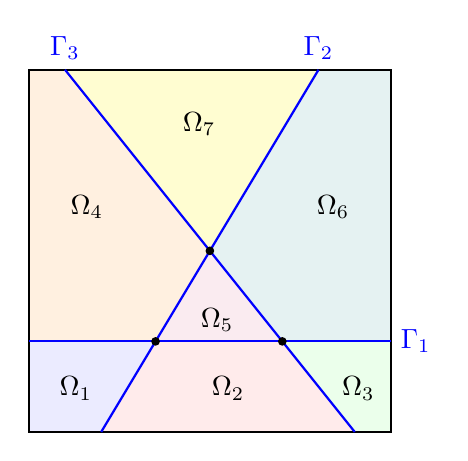
\begin{tikzpicture}[x=4.6cm,y=4.6cm]
  % Panel (a): three boundary-to-boundary fractures -> 7 subregions.
  \coordinate (L1)  at (0,0.25);
  \coordinate (R1)  at (1,0.25);
  \coordinate (B2)  at (0.20,0);
  \coordinate (T2)  at (0.80,1);
  \coordinate (B3)  at (0.90,0);
  \coordinate (T3)  at (0.10,1);
  \coordinate (P12) at (0.35,0.25);
  \coordinate (P13) at (0.70,0.25);
  \coordinate (P23) at (0.50,0.50);

  \fill[blue!8]    (0,0) -- (B2) -- (P12) -- (L1) -- cycle;
  \fill[red!8]     (B2) -- (B3) -- (P13) -- (P12) -- cycle;
  \fill[green!8]   (B3) -- (1,0) -- (R1) -- (P13) -- cycle;
  \fill[orange!12] (L1) -- (P12) -- (P23) -- (T3) -- (0,1) -- cycle;
  \fill[purple!8]  (P12) -- (P13) -- (P23) -- cycle;
  \fill[teal!10]   (R1) -- (1,1) -- (T2) -- (P23) -- (P13) -- cycle;
  \fill[yellow!18] (P23) -- (T2) -- (T3) -- cycle;

  \draw[thick] (0,0) rectangle (1,1);
  \draw[thick,blue] (L1) -- (R1);
  \draw[thick,blue] (B2) -- (T2);
  \draw[thick,blue] (B3) -- (T3);

  \fill (P12) circle (0.012);
  \fill (P13) circle (0.012);
  \fill (P23) circle (0.012);

  \node[blue,right] at (R1) {\(\Gamma_1\)};
  \node[blue,above] at (T2) {\(\Gamma_2\)};
  \node[blue,above] at (T3) {\(\Gamma_3\)};

  \node at (0.13,0.12) {\(\Omega_1\)};
  \node at (0.55,0.12) {\(\Omega_2\)};
  \node at (0.91,0.12) {\(\Omega_3\)};
  \node at (0.16,0.62) {\(\Omega_4\)};
  \node at (0.52,0.31) {\(\Omega_5\)};
  \node at (0.84,0.62) {\(\Omega_6\)};
  \node at (0.47,0.85) {\(\Omega_7\)};
\end{tikzpicture}
\par\smallskip\small (a)
\end{minipage}
\hfill
\begin{minipage}{0.48\textwidth}
\centering
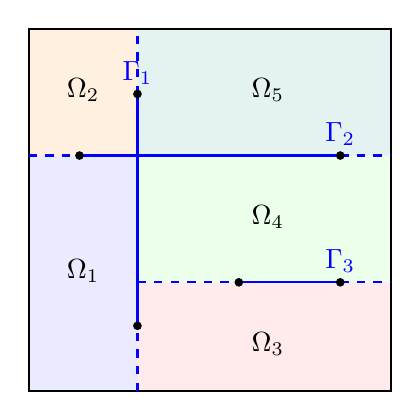
\begin{tikzpicture}[x=4.6cm,y=4.6cm]
  % Panel (b): three interior fractures with ghost extensions.

  \coordinate (A1) at (0.30,0.18);
  \coordinate (B1) at (0.30,0.82);
  \coordinate (A2) at (0.14,0.65);
  \coordinate (B2) at (0.86,0.65);
  \coordinate (A3) at (0.58,0.30);
  \coordinate (B3) at (0.86,0.30);

  \fill[blue!8]    (0,0)       rectangle (0.30,0.65);
  \fill[orange!12] (0,0.65)    rectangle (0.30,1);
  \fill[red!8]     (0.30,0)    rectangle (1,0.30);
  \fill[green!8]   (0.30,0.30) rectangle (1,0.65);
  \fill[teal!10]   (0.30,0.65) rectangle (1,1);

  \draw[thick] (0,0) rectangle (1,1);

  \draw[thick,blue,dashed] (0.30,0) -- (A1);
  \draw[thick,blue]        (A1) -- (B1);
  \draw[thick,blue,dashed] (B1) -- (0.30,1);

  \draw[thick,blue,dashed] (0,0.65) -- (A2);
  \draw[thick,blue]        (A2) -- (B2);
  \draw[thick,blue,dashed] (B2) -- (1,0.65);

  \draw[thick,blue,dashed] (0.30,0.30) -- (A3);
  \draw[thick,blue]        (A3) -- (B3);
  \draw[thick,blue,dashed] (B3) -- (1,0.30);

  \fill (A1) circle (0.012);
  \fill (B1) circle (0.012);
  \fill (A2) circle (0.012);
  \fill (B2) circle (0.012);
  \fill (A3) circle (0.012);
  \fill (B3) circle (0.012);

  \node[blue,above] at (B1) {\(\Gamma_1\)};
  \node[blue,above] at (B2) {\(\Gamma_2\)};
  \node[blue,above] at (B3) {\(\Gamma_3\)};

  \node at (0.15,0.33) {\(\Omega_1\)};
  \node at (0.15,0.83) {\(\Omega_2\)};
  \node at (0.66,0.13) {\(\Omega_3\)};
  \node at (0.66,0.48) {\(\Omega_4\)};
  \node at (0.66,0.83) {\(\Omega_5\)};
\end{tikzpicture}
\par\smallskip\small (b)
\end{minipage}
\captionof{figure}{Partition of the matrix domain \(\Omega\) by the fracture
network into subregions \(\Omega_r\), each assigned its own flux network
\(\mathbf{v}_{\theta,r}\). (a) Three pairwise-intersecting boundary-to-boundary
fractures give \(N_s=1+N_\Gamma+N_\Gamma(N_\Gamma-1)/2=7\) subregions. (b) Three finite
fractures are completed by dashed ghost interfaces so the switching partition has
\(N_s=1+N_\Gamma+N_I=1+3+1=5\) subregions. The ghost interfaces only extend the
side-network partition and carry zero jump target.}
\label{fig:subregion_partition}
\end{center}

For a single fracture, the partition reduces to the two sides \(\Omega^+\) and
\(\Omega^-\) of Figure~\ref{fig:fracture_schematic}, with the two-network
representation \(\vflux_\theta^+\) and \(\vflux_\theta^-\). With
\(\mathbf{n}_\Gamma\) oriented from the minus side to the plus side, the
representation is smooth on each side but permits a prescribed normal flux jump
on \(\Gamma\). In the LMDFM setting, this physical jump equals the discrete
multiplier,
\(\jump{\vflux\cdot\mathbf{n}_\Gamma}\approx\lambda_h\), under the orientation
convention fixed in Section~\ref{sec:model-diagnostics}. In a fracture network,
the same idea is applied locally: physical fracture pieces carry the
multiplier-driven jump, while ghost interfaces carry a zero jump target.

Once the subregions are defined, the networks
\(\{\vflux_{\theta,r}\}_{r=1}^{N_s}\) are trained jointly by minimizing a single
fractured-domain loss,
\begin{equation}
\mathcal{L}
=
w_d\mathcal{L}_d
+
w_{\nabla\cdot}\mathcal{L}_{\nabla\cdot}
+
w_j\mathcal{L}_j
+
w_g\mathcal{L}_g
+
w_c\mathcal{L}_c .
\label{eq:pinn_fractured_loss}
\end{equation}
Its five terms, balanced by the weights \(w_\bullet\), fall into three groups:
two interior terms that act away from the fractures (the data term
\(\mathcal{L}_d\) and the divergence term \(\mathcal{L}_{\nabla\cdot}\)), two
interface terms that act on the fractures (the physical-jump term
\(\mathcal{L}_j\) and the ghost-jump term \(\mathcal{L}_g\)), and a balance term
\(\mathcal{L}_c\) on the fracture-cut elements. We take them in turn.

Away from the fractures the raw CG flux is smooth and accurate and provides a
reliable training target. Near a fracture, whether \(\vflux_h\) stays reliable depends on the
mesh. On a nonconforming mesh the fracture cuts through elements, where the
continuous \(\vflux_h\) cannot represent the jump and averages the two sides; the
data on those cut cells is then unreliable and must be excluded. On a conforming
mesh, by contrast, the fracture lies on facets and its jump is carried exactly by
\(\lambda_h\), so \(\vflux_h\) is one-sided and valid up to the interface, and no
such exclusion is needed. The divergence
term is dropped in a band around every fracture either way, since
\(\nabla\cdot\vflux=f\) is ill-posed there through the matrix--fracture exchange;
the cut-element balance \(\mathcal{L}_c\) below restores conservation. With \(h\) the matrix
mesh size and
\(m>0\) setting the band width \(mh\) around every physical and ghost interface,
\[
  \mathcal{B}_h
  =
  \left\{\mathbf{x}\in\Omega:
  \min_{\mathbf{y}\in\Gamma\cup\Gamma^{\mathrm{g}}}\|\mathbf{x}-\mathbf{y}\|\le mh
  \right\},
  \qquad
  \Gamma^{\mathrm{g}}=\cup_{\ell=1}^{N_\Gamma}
  \Gamma_\ell^{\mathrm{g}} ,
\]
the divergence term is evaluated outside \(\mathcal{B}_h\); so is
the data term on a nonconforming mesh, but over all of \(\Omega\) on a conforming
one,
\begin{equation}
\mathcal{L}_d
=
\frac{1}{N_d}\sum_{i=1}^{N_d}
\|\vflux_\theta(\mathbf{x}_i^d)-\vflux_h(\mathbf{x}_i^d)\|^2,
\qquad
\mathcal{L}_{\nabla\cdot}
=
\frac{1}{N_f}\sum_{i=1}^{N_f}
\left|\nabla\cdot\vflux_\theta(\mathbf{x}_i^f)-f(\mathbf{x}_i^f)\right|^2 .
\label{eq:pinn_data_div_loss}
\end{equation}

Across each fracture the two adjacent networks must first be identified. On a
physical segment \(\Gamma_\ell\), let \(r_\ell^+\) and \(r_\ell^-\) index the
subregions on its two sides and let \(\mathbf{n}_\ell\) point from
\(\Omega_{r_\ell^-}\) to \(\Omega_{r_\ell^+}\); the physical-jump term then forces
the normal jump of the reconstructed flux to equal the LMDFM multiplier,
\begin{equation}
\mathcal{L}_j
=
\frac{1}{N_j}
\sum_{\ell=1}^{N_\Gamma}
\sum_{\mathbf{x}_q\in\mathcal{X}_\ell^j}
\left|
\left(
\vflux_{\theta,r_\ell^+}(\mathbf{x}_q)
-
\vflux_{\theta,r_\ell^-}(\mathbf{x}_q)
\right)\cdot\mathbf{n}_\ell
-
\lambda_h(\mathbf{x}_q)
\right|^2 .
\label{eq:pinn_jump_loss}
\end{equation}
Here \(\mathcal{X}_\ell^j\subset\Gamma_\ell\) collects the jump collocation points
and \(N_j=\sum_\ell|\mathcal{X}_\ell^j|\). This is the fracture analogue of the
interface conditions used in conservative PINNs \citep{Jagtap2020}, except that the target is the
multiplier-driven jump \(\lambda_h\) rather than zero. The ghost-jump term applies
the same operator on the ghost interfaces with target zero,
\begin{equation}
\mathcal{L}_g
=
\frac{1}{N_g}
\sum_{\ell=1}^{N_\Gamma}
\sum_{\mathbf{x}_q\in\mathcal{X}_\ell^g}
\left|
\left(
\vflux_{\theta,r_\ell^+}(\mathbf{x}_q)
-
\vflux_{\theta,r_\ell^-}(\mathbf{x}_q)
\right)\cdot\mathbf{n}_\ell
\right|^2 ,
\label{eq:pinn_ghost_loss}
\end{equation}
where \(\mathcal{X}_\ell^g\subset\Gamma_\ell^{\mathrm{g}}\) and
\(N_g=\sum_\ell|\mathcal{X}_\ell^g|\); it is omitted when no ghost interface is
present.

Finally, since the exclusion band removed the fracture-cut elements from the
divergence term, those elements are left without any conservation constraint. We
restore one there in integrated form---penalizing on each cut element the mass
balance \(R_\tau\) of \eqref{eq:element_residual}, a boundary-flux balance that
stays well defined even where the flux jumps inside the element,
\begin{equation}
\mathcal{L}_c
=
\frac{1}{|\mathcal{T}_\Gamma|}
\sum_{\tau\in\mathcal{T}_\Gamma}
\left(
\frac{R_\tau(\vflux_\theta,\lambda_h)}
{\max(|R_\tau(\vflux_h,\lambda_h)|,\varepsilon)}
\right)^2,
\label{eq:pinn_element_loss}
\end{equation}
over the cut elements
\(\mathcal{T}_\Gamma=\{\tau\in\mathcal{T}_h:\tau\cap\Gamma\ne\emptyset\}\), with
\(\varepsilon>0\) guarding against division by zero. The balance is written here on
the flow-mesh elements \(\tau\), but the same integrated constraint can be imposed
on any control volume---nodal dual volumes or other control volumes---not only
mesh elements. Normalizing each residual by its raw CG value
\(R_\tau(\vflux_h,\lambda_h)\), rather than penalizing \(R_\tau(\vflux_\theta)\)
directly, makes the term dimensionless and scale-invariant: it measures the
relative improvement over the CG defect on the same element, so that elements with
large fluxes or sources do not dominate the loss and the network is driven to
reduce the defect proportionally everywhere.

Each subregion network \(\vflux_{\theta,r}\) is a fully connected feedforward network
with \(L\) hidden layers and width \(W\). The activation is written
\(\sigma(a\,\cdot)\), where \(a\) is a trainable scalar slope initialized to one
and optimized together with the weights. This adaptive activation follows the
strategy used in conservative PINNs \citep{Jagtap2020} and improves training
robustness relative to a fixed activation scale. At exact convergence the PINN
enforces \(\nabla\cdot\vflux_{\theta,r}=f\),
\(\jump{\vflux_\theta\cdot\mathbf{n}}=\lambda_h\) on physical fractures, zero
jump on ghost interfaces, and \(R_\tau(\vflux_\theta,\lambda_h)=0\) on the
constrained elements away from tips and intersections. In practice these
conditions hold only approximately, so we report \(R_\tau\), \(R_\xi\), and,
where needed, mesh-independent diagnostics such as \(R_\zeta\).

{\color{red}
\noindent\textbf{TODO (item to add, expect ~1 page):}
\begin{itemize}
\item PINN conservation bound (divergence theorem): for any control volume \(\omega\), the conservation defect \(R_\omega\) obeys \(|R_\omega|\lesssim ...\) (should correspond to $\nabla \cdot \vflux_{\theta} - f$ consistent with the observed \(R_\tau,R_\xi,R_\zeta\) of the same order); the \emph{a~posteriori} analogue of the exact NLR identity \(R_\xi=0\) (Prop.~\ref{prop:dual-volume-conservation}).
\end{itemize}
}

We expect the PINN to be most attractive in the coupled time-dependent problem,
where the flux must be reconstructed at every time step. Between consecutive steps
the pressure---and hence the target flux---changes only slightly, so the network
trained at step \(n\) should be an excellent initial guess for step \(n+1\):
re-using its weights (warm starting) should reduce the per-step training to a few
optimizer iterations, rather than the cold-start cost of a single steady solve.
The deterministic NLR, by contrast, is recomputed from scratch at each step,
though its element-local solves are individually inexpensive. Our hypothesis is
therefore that the time-dependent setting amortizes the PINN's main
weakness---its training cost---over the simulation, so that the PINN becomes
competitive there while keeping its pointwise-conservation and
general-control-volume advantages. When \(\Kmat\) is independent of \(S\) the flux
is reconstructed once and frozen, and this advantage does not arise.

A single network over a whole subregion must represent two very different fields
at once: the smooth flux in the interior and the sharp, multiplier-driven jump
along the fracture. Forcing one network to capture both makes training harder and
spends capacity where it is not needed. We therefore decompose each subregion,
following the conservative PINN (cPINN) idea of \citet{Jagtap2020}, in which the
domain is split into pieces that each carry their own network and are coupled
through interface flux-continuity.

We split each subregion \(\Omega_r\) into an interior piece \(\Omega_{r,0}\)---the
part of \(\Omega_r\) outside the band \(\mathcal{B}_h\) ---and one boundary piece \(\Omega_{r,j}\) for each bounding
fracture or ghost segment \(\Gamma_j\) (Figure~\ref{fig:cpinn_partition}). The
second subscript labels the piece: \(0\) is the interior, and \(j\) is the
boundary band attached to \(\Gamma_j\). Because the interior and boundary networks
now meet at the band edge \(\partial\mathcal{B}_h\cap\Omega_r\), we add an
interior--boundary flux-continuity term that keeps the reconstructed flux
single-valued there,
\begin{equation}
\mathcal{L}_b
=
\frac{1}{N_b}\sum_{\mathbf{x}_q\in\mathcal{X}_b}
\bigl|\jump{\vflux_\theta\cdot\mathbf{n}}(\mathbf{x}_q)\bigr|^2 ,
\qquad
\mathcal{X}_b\subset\partial\mathcal{B}_h\cap\Omega_r ,
\label{eq:pinn_band_continuity}
\end{equation}
the same zero-jump interface condition that \(\mathcal{L}_j\) and \(\mathcal{L}_g\)
impose across the fractures. At a fracture intersection, the two boundary bands of a
subregion follow the crossing fractures and meet in the corner; we separate them
along the diagonal that bisects that corner (the dashed lines in
Figure~\ref{fig:cpinn_partition}), giving each band the side facing its own
fracture, and impose the same zero-jump continuity across this diagonal. The
collocation set \(\mathcal{X}_b\) therefore collects every internal seam of the
sub-partition: the edges between an interior network and its boundary bands, and
the diagonal seams between two boundary bands at an intersection.

\begin{center}
\centering
\resizebox{0.6\linewidth}{!}{%
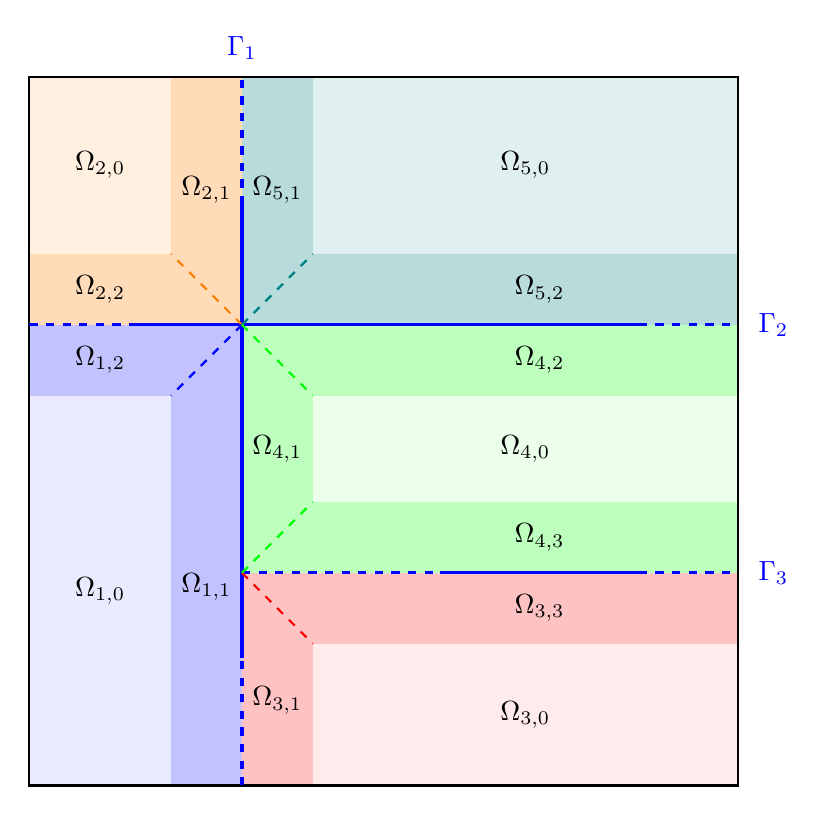
\begin{tikzpicture}[x=9cm,y=9cm,>=Stealth]
  \color{black}% keep the figure black even when placed inside the orange block
  % cPINN sub-partition of the five-subregion (ghost) case of
  % Figure~\ref{fig:subregion_partition}(b). Interiors (light) + boundary bands
  % (darker), one colour family per subregion. Bands drawn exaggerated.
  % Gamma_1: x=0.30 (vertical); Gamma_2: y=0.65; Gamma_3: y=0.30 (x>=0.30).
  % Omega_1 [0,0.30]x[0,0.65] : Gamma_1 right, Gamma_2 top
  \fill[blue!8]   (0,0) rectangle (0.20,0.55);
  \fill[blue!24]  (0.20,0) rectangle (0.30,0.65);
  \fill[blue!24]  (0,0.55) rectangle (0.20,0.65);
  % Omega_2 [0,0.30]x[0.65,1] : Gamma_1 right, Gamma_2 bottom
  \fill[orange!12] (0,0.75) rectangle (0.20,1);
  \fill[orange!28] (0.20,0.65) rectangle (0.30,1);
  \fill[orange!28] (0,0.65) rectangle (0.20,0.75);
  % Omega_3 [0.30,1]x[0,0.30] : Gamma_1 left, Gamma_3 top
  \fill[red!8]    (0.40,0) rectangle (1,0.20);
  \fill[red!24]   (0.30,0) rectangle (0.40,0.30);
  \fill[red!24]   (0.40,0.20) rectangle (1,0.30);
  % Omega_4 [0.30,1]x[0.30,0.65] : Gamma_1 left, Gamma_3 bottom, Gamma_2 top
  \fill[green!8]  (0.40,0.40) rectangle (1,0.55);
  \fill[green!26] (0.30,0.30) rectangle (0.40,0.65);
  \fill[green!26] (0.40,0.30) rectangle (1,0.40);
  \fill[green!26] (0.40,0.55) rectangle (1,0.65);
  % Omega_5 [0.30,1]x[0.65,1] : Gamma_1 left, Gamma_2 bottom
  \fill[teal!12]  (0.40,0.75) rectangle (1,1);
  \fill[teal!28]  (0.30,0.65) rectangle (0.40,1);
  \fill[teal!28]  (0.40,0.65) rectangle (1,0.75);

  \draw[thick] (0,0) rectangle (1,1);

  % fractures (solid) with ghost extensions (dashed)
  \draw[very thick,blue,dashed] (0.30,0) -- (0.30,0.18);
  \draw[very thick,blue]        (0.30,0.18) -- (0.30,0.82);
  \draw[very thick,blue,dashed] (0.30,0.82) -- (0.30,1);
  \draw[very thick,blue,dashed] (0,0.65) -- (0.14,0.65);
  \draw[very thick,blue]        (0.14,0.65) -- (0.86,0.65);
  \draw[very thick,blue,dashed] (0.86,0.65) -- (1,0.65);
  \draw[very thick,blue,dashed] (0.30,0.30) -- (0.58,0.30);
  \draw[very thick,blue]        (0.58,0.30) -- (0.86,0.30);
  \draw[very thick,blue,dashed] (0.86,0.30) -- (1,0.30);

  % diagonal corner separators between the two boundary bands of a subregion
  % at a fracture intersection (each carries the continuity term L_b);
  % dashed, in the same colour as the subregion it lies in
  \draw[thick,dashed,orange] (0.30,0.65) -- (0.20,0.75);  % into Omega_2
  \draw[thick,dashed,teal]   (0.30,0.65) -- (0.40,0.75);  % into Omega_5
  \draw[thick,dashed,blue]   (0.30,0.65) -- (0.20,0.55);  % into Omega_1
  \draw[thick,dashed,green]  (0.30,0.65) -- (0.40,0.55);  % into Omega_4
  \draw[thick,dashed,red]    (0.30,0.30) -- (0.40,0.20);  % into Omega_3
  \draw[thick,dashed,green]  (0.30,0.30) -- (0.40,0.40);  % into Omega_4

  \node[blue] at (0.30,1.04) {\(\Gamma_1\)};
  \node[blue] at (1.05,0.65) {\(\Gamma_2\)};
  \node[blue] at (1.05,0.30) {\(\Gamma_3\)};

  % region labels (body font, horizontal)
  \node at (0.10,0.275) {\(\Omega_{1,0}\)};
  \node at (0.10,0.875) {\(\Omega_{2,0}\)};
  \node at (0.70,0.10)  {\(\Omega_{3,0}\)};
  \node at (0.70,0.475) {\(\Omega_{4,0}\)};
  \node at (0.70,0.875) {\(\Omega_{5,0}\)};

  \node at (0.25,0.28)  {\(\Omega_{1,1}\)};
  \node at (0.25,0.84)  {\(\Omega_{2,1}\)};
  \node at (0.35,0.12)  {\(\Omega_{3,1}\)};
  \node at (0.35,0.475) {\(\Omega_{4,1}\)};
  \node at (0.35,0.84)  {\(\Omega_{5,1}\)};

  \node at (0.10,0.60) {\(\Omega_{1,2}\)};
  \node at (0.10,0.70) {\(\Omega_{2,2}\)};
  \node at (0.72,0.25) {\(\Omega_{3,3}\)};
  \node at (0.72,0.35) {\(\Omega_{4,3}\)};
  \node at (0.72,0.60) {\(\Omega_{4,2}\)};
  \node at (0.72,0.70) {\(\Omega_{5,2}\)};
\end{tikzpicture}%
}
\captionof{figure}{cPINN sub-partition of the five subregions of
Figure~\ref{fig:subregion_partition}(b). Each subregion \(\Omega_r\) is split into
an interior network \(\Omega_{r,0}\) (lighter shade), trained on the data and
divergence terms, and one boundary network \(\Omega_{r,j}\) (darker shade) per
bounding fracture or ghost segment \(\Gamma_j\), trained on the
jump, balance, and data terms; the colour groups the networks belonging to one
subregion. Bands are drawn exaggerated for clarity. The interior--boundary
interfaces between \(\Omega_{r,0}\) and the \(\Omega_{r,j}\), and the dashed
diagonal separators between two boundary bands meeting at a fracture
intersection, all carry the continuity term \(\mathcal{L}_b\).}
\label{fig:cpinn_partition}
\end{center}

We then size each network to the field it must represent. On the interior the
flux $\Omega_{r,0}$ is smooth and already well approximated by $\vflux_h$, so a small,
shallow network suffices; it is trained on the data and divergence terms together
with the shared continuity term,
\begin{equation}
\mathcal{L}_{r,0}
=
w_d\mathcal{L}_d+w_{\nabla\cdot}\mathcal{L}_{\nabla\cdot}+w_b\mathcal{L}_b .
\end{equation}
Each boundary network must instead resolve the jump, so it is deeper and wider.
The data term still anchors it to \(\vflux_h\) wherever \(\vflux_h\)
is valid (the whole band when conforming, outside the cut cells otherwise),
alongside the interface, balance, and continuity terms,
\begin{equation}
\mathcal{L}_{r,j}
=
w_d\mathcal{L}_d+w_j\mathcal{L}_j+w_g\mathcal{L}_g+w_c\mathcal{L}_c+w_b\mathcal{L}_b .
\end{equation}

We use one boundary band per subregion along each fracture or ghost segment, so a
subregion with \(b\) bounding segments carries \(1+b\) networks. Confining
the rich, jump-resolving capacity to the thin boundary bands while keeping a cheap
interior network is what lets the cPINN lower the training cost relative to a
single large network over the whole subregion, at the same conservation
guarantees.

The decomposition also makes training parallel. The data, divergence, and balance
terms \(\mathcal{L}_d,\mathcal{L}_{\nabla\cdot},\mathcal{L}_c\) are local to one
network, so networks couple only through the interface terms
\(\mathcal{L}_j,\mathcal{L}_g,\mathcal{L}_b\), and only between neighbours. Each
network can therefore train independently, exchanging with each neighbour only the
normal flux \(\vflux_\theta\cdot\mathbf{n}\) sampled on their shared interface---a
small nearest-neighbour communication, not a global one. The coupling can also be staged: since every
\(\vflux_\theta\) is anchored to \(\vflux_h\) by its data term and the jump targets
(\(\lambda_h\), or zero) are known from the CG solve, the interface terms only
correct an already near-consistent field. One may thus train in parallel with the
continuity terms off, or ramped, and enforce them only as a final reconciliation
once the residual jumps are small. With warm starting across time steps, this
keeps the per-step cost low.

\subsection{\textcolor{orange}{Local conservation of the fracture flux}}
\label{subsec:fracture-flux}

{\color{orange}
Both matrix-flux reconstructions of the previous subsections---the deterministic
NLR (Section~\ref{subsec:nlr}) and the PINN
(Section~\ref{subsec:pinn-reconstruction})---act on the two-dimensional matrix
flux; the one-dimensional fracture flux is common to both. Here we fix that
fracture flux, establish its local conservation, and then explain why an
element-local reconstruction is not applied to it.

The fracture transport update consumes one tangential flux per face of the fracture
mesh, and two quantities are available from the CG-LMDFM fracture pressure
\(p_{\Gamma,h}\). The first is the finite-element element-gradient flux
\[
  \vflux_{\Gamma,h}=-K_\Gamma\,\partial_s p_{\Gamma,h},
\]
a per-element field, constant on each element for piecewise-linear pressure. The
second is the two-point (TPFA) face flux between adjacent nodes \(j\) and \(j+1\),
\[
  u_{\Gamma,j+1/2}=-K_{\Gamma,j+1/2}\,
  \frac{p_{\Gamma,j+1}-p_{\Gamma,j}}{\ell_{\Gamma,j+1/2}},
\]
with \(K_{\Gamma,j+1/2}/\ell_{\Gamma,j+1/2}\) the transmissibility of the element
between nodes \(j\) and \(j+1\), of length \(\ell_{\Gamma,j+1/2}=x_{j+1}-x_j\) and
conductivity \(K_{\Gamma,j+1/2}\). The half-integer index marks the inter-nodal
element and the face at its midpoint, so node \(j\) is flanked by elements of lengths
\(\ell_{\Gamma,j-1/2}\) and \(\ell_{\Gamma,j+1/2}\). For piecewise-linear pressure the
element gradient
on \([x_j,x_{j+1}]\) is exactly
\(-K_\Gamma(p_{\Gamma,j+1}-p_{\Gamma,j})/\ell_{\Gamma,j+1/2}\), so the two definitions
coincide on every face; they differ only for \(k\ge2\), where \(\vflux_{\Gamma,h}\)
carries the interior polynomial modes while \(u_{\Gamma,j+1/2}\) uses the endpoint
values alone. Being single-valued per face, the two-point flux is the one the
transport update uses.

\begin{center}
\centering
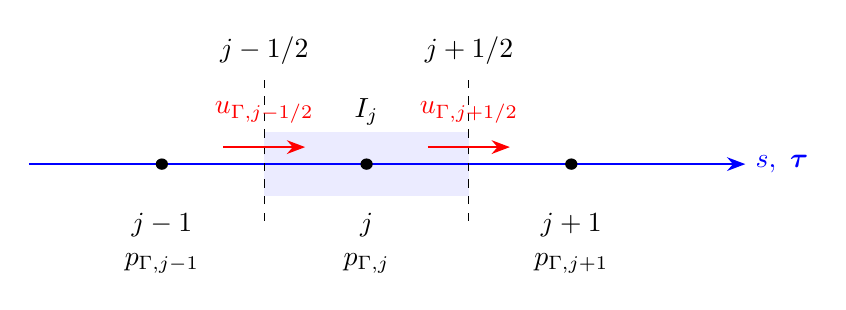
\begin{tikzpicture}[>=Stealth,x=1.3cm,y=1.2cm]
  \color{black}% keep the diagram black inside the orange block
  % node-centred control volume I_j (the dual cell)
  \fill[blue!8] (-1,-0.34) rectangle (1,0.34);
  % fracture line, arclength s / tangent tau
  \draw[thick,blue] (-3.3,0) -- (3.0,0);
  \draw[->,thick,blue] (3.0,0) -- (3.7,0) node[right] {$s,\ \bm\tau$};
  % faces (dual-cell boundaries) at the element midpoints
  \draw[dashed] (-1,-0.6) -- (-1,0.95);
  \draw[dashed] ( 1,-0.6) -- ( 1,0.95);
  \node[above] at (-1,0.95) {$j-1/2$};
  \node[above] at ( 1,0.95) {$j+1/2$};
  % nodes (fracture-pressure DOFs)
  \fill (-2,0) circle (0.06);
  \fill ( 0,0) circle (0.06);
  \fill ( 2,0) circle (0.06);
  \node[below,align=center] at (-2,-0.42) {$j-1$\\$p_{\Gamma,j-1}$};
  \node[below,align=center] at ( 0,-0.42) {$j$\\$p_{\Gamma,j}$};
  \node[below,align=center] at ( 2,-0.42) {$j+1$\\$p_{\Gamma,j+1}$};
  % two-point face fluxes (positive in +s)
  \draw[->,thick,red] (-1.4,0.18) -- (-0.6,0.18);
  \draw[->,thick,red] ( 0.6,0.18) -- ( 1.4,0.18);
  \node[red] at (-1,0.55) {$u_{\Gamma,j-1/2}$};
  \node[red] at ( 1,0.55) {$u_{\Gamma,j+1/2}$};
  % cell name
  \node at (0,0.55) {$I_j$};
\end{tikzpicture}
\captionof{figure}{One-dimensional fracture stencil. The node-centred control volume
\(I_j\) (shaded) spans the two faces \(j\mp1/2\) at the midpoints of the elements
adjoining node \(j\). The two-point face fluxes \(u_{\Gamma,j\mp1/2}\) (red), each
formed from the two adjacent nodal pressures \(p_{\Gamma,\bullet}\), give the net
tangential outflow \(u_{\Gamma,j+1/2}-u_{\Gamma,j-1/2}\) that the Proposition equates
to the fracture source and the matrix--fracture exchange over \(I_j\).}
\label{fig:fracture_stencil}
\end{center}

The local-conservation requirement is the one-dimensional analogue of the element
residual \eqref{eq:element_residual}: integrating the fracture pressure equation
\eqref{eq:lmdfm_strong} over the node-centred control volume \(I_j\) of node \(j\)
(the interval between the midpoints of the two adjacent elements;
Figure~\ref{fig:fracture_stencil}) gives
\begin{equation}
\int_{\partial I_j}\vflux_{\Gamma,h}\cdot\bm\tau
=
\int_{I_j} f_\Gamma - \int_{I_j}\lambda_h ,
\label{eq:fracture_balance}
\end{equation}
the net tangential outflow balancing the fracture source and the matrix--fracture
exchange (with the effective source of Section~\ref{subsec:nlr} in the parabolic
case). The two-point flux supplies the boundary term as
\(\int_{\partial I_j}\vflux_{\Gamma,h}\cdot\bm\tau=u_{\Gamma,j+1/2}-u_{\Gamma,j-1/2}\),
so local conservation reduces to the following.

\begin{proposition}[Local conservation of the CG fracture flux]
\label{prop:fracture-conservation}
Let the fracture pressure be piecewise linear with nodal hat basis
\(\{\phi_{\Gamma,j}\}\), and let \(f_\Gamma\) and \(\lambda_h\) be piecewise
constant on the fracture mesh. Then on every interior fracture node \(j\),
\[
  u_{\Gamma,j+1/2}-u_{\Gamma,j-1/2}
  =
  \int_\Gamma\bigl(f_\Gamma-\lambda_h\bigr)\,\phi_{\Gamma,j}\,\dd s .
\]
Hence the two-point fracture flux is locally conservative on every interior cell
\(I_j\).
\end{proposition}

\noindent\emph{Proof.}
Test the discrete system \eqref{eq:lmdfm_cg} with
\((q_h,q_{\Gamma,h},\mu_h)=(0,\phi_{\Gamma,j},0)\). The terms in \(q_h\) drop and the
coupling term gives \(-\int_\Gamma\lambda_h(0-\phi_{\Gamma,j})\), leaving
\[
  \int_\Gamma K_\Gamma\,\partial_s p_{\Gamma,h}\,\partial_s\phi_{\Gamma,j}
  +\int_\Gamma\lambda_h\,\phi_{\Gamma,j}
  =\int_\Gamma f_\Gamma\,\phi_{\Gamma,j}.
\]
The hat \(\phi_{\Gamma,j}\) is supported on the two elements adjacent to node \(j\):
on the left element \([x_{j-1},x_j]\) of length \(\ell_{\Gamma,j-1/2}\) its slope is
\(\partial_s\phi_{\Gamma,j}=+1/\ell_{\Gamma,j-1/2}\), and on the right element
\([x_j,x_{j+1}]\) of length \(\ell_{\Gamma,j+1/2}\) it is \(-1/\ell_{\Gamma,j+1/2}\).
Evaluate the conductivity at the two faces, \(K_{\Gamma,j-1/2}\) and
\(K_{\Gamma,j+1/2}\)---the values already carried by the two-point fluxes---and
recall that \(\partial_s p_{\Gamma,h}\) is the constant element slope of the
piecewise-linear pressure. The contribution of each element is then
\(K_{\Gamma,j\mp1/2}\) times the product of the two constant slopes times the element
length, and the length cancels the \(1/\ell\) carried by the basis slope, leaving
exactly one two-point face flux per element,
\[
  \int_{x_{j-1}}^{x_j} K_\Gamma\,\partial_s p_{\Gamma,h}\,\partial_s\phi_{\Gamma,j}
  =K_{\Gamma,j-1/2}\,\frac{p_{\Gamma,j}-p_{\Gamma,j-1}}{\ell_{\Gamma,j-1/2}}
  =-\,u_{\Gamma,j-1/2},
\]
\[
  \int_{x_j}^{x_{j+1}} K_\Gamma\,\partial_s p_{\Gamma,h}\,\partial_s\phi_{\Gamma,j}
  =-\,K_{\Gamma,j+1/2}\,\frac{p_{\Gamma,j+1}-p_{\Gamma,j}}{\ell_{\Gamma,j+1/2}}
  =u_{\Gamma,j+1/2}.
\]
Since \(\phi_{\Gamma,j}\) vanishes outside these two elements,
\(\int_\Gamma=\int_{x_{j-1}}^{x_j}+\int_{x_j}^{x_{j+1}}\), so adding the two lines
gives
\[
  \int_\Gamma K_\Gamma\,\partial_s p_{\Gamma,h}\,\partial_s\phi_{\Gamma,j}
  =u_{\Gamma,j+1/2}-u_{\Gamma,j-1/2},
\]
and substituting into the tested equation yields the identity. The right-hand side
then simplifies because \(f_\Gamma\) and \(\lambda_h\) are piecewise constant: on
each element adjacent to node \(j\) the hat \(\phi_{\Gamma,j}\) integrates to half
the element length (its triangle area \(\tfrac12\ell_{\Gamma,j\mp1/2}\)), which is
exactly the part of the dual cell \(I_j\) lying in that element, so a constant
integrand contributes the same either way and the hat-weighted integral equals the
plain cell integral,
\(\int_\Gamma(f_\Gamma-\lambda_h)\phi_{\Gamma,j}=\int_{I_j}(f_\Gamma-\lambda_h)\).
Hence the two-point flux on the control volume \(I_j\) satisfies
\[
u_{\Gamma,j+1/2}-u_{\Gamma,j-1/2}=\int_{\partial I_j}\vflux_{\Gamma,h}\cdot\bm\tau
=\int_{I_j}\bigl(f_\Gamma-\lambda_h\bigr),
\]
the cell balance \eqref{eq:fracture_balance}, and is locally conservative on
\(I_j\). \(\square\)

The identity of the Proposition is precisely the dual-volume balance that the matrix
reconstruction is
constructed to enforce (Proposition~\ref{prop:dual-volume-conservation}, with the
fracture cell \(I_j\) in place of the nodal dual volume \(C^\xi\)). Both
reconstruction routes exist to restore this control-volume balance where the raw
flux lacks it, and on the fracture the two-point flux already provides it, so
neither is needed for the transport. The one-dimensional analogue of the
element-local problem \eqref{eq:nlr_local_problem} would re-solve for a flux already
in hand, returning the same field up to the constant null space. A PINN would
instead enforce the divergence pointwise, conserving on arbitrary control volumes as
it does on the matrix, and it extends to the fracture flux in the same way. We do
not pursue this here: the focus of this work is the matrix flux reconstruction, so we
keep the fracture flux fixed---the conservative two-point scheme---across all routes
(raw CG, NLR, and PINN), and any difference in the transport then reflects the matrix
reconstruction alone rather than a change in the fracture flux.

The matrix flux, by contrast, must be reconstructed: the exact control-volume
balance of the Proposition is special to one dimension, and the two-dimensional CG
flux, read on the same control volumes, does not satisfy it---its control-volume
residual \(R_\xi\) is nonzero, the lack of local conservation that motivates this
work. We therefore reconstruct the matrix flux only and take the two-point fracture
flux directly, in both the NLR and PINN routes.

Two further points delimit the result. First, it is specific to \(k=1\): for
\(k\ge2\) the element-gradient and two-point fluxes no longer coincide so a genuine reconstruction would be
needed, the construction of Section~\ref{subsec:nlr} with \(\nabla\) replaced by
\(\partial_s\) and the exchange entering as a distributed source
\(f_\Gamma-\lambda_h\) rather than a concentrated one (hence without the split
weights and consistency lemma of the matrix case). Accordingly the transport
experiments use \(k=1\) fracture pressure, matched to the first-order upwind
finite-volume scheme, while the higher-degree runs of
Section~\ref{subsec:single-fracture-benchmark} are pressure-convergence studies that
make no fracture-flux conservation claim. Second, the same multiplier \(\lambda_h\)
enters the matrix balance as a source and the fracture balance as a sink, so the two
exchange contributions cancel and global mass is conserved.
}

\subsection{Coupled flow--transport algorithm}
\label{subsec:method-coupling}

The pieces above assemble into a single sequential time-stepping scheme. Given
the saturation \(S^n\) at time \(t^n\), one step proceeds as follows.
\begin{enumerate}
\item Assemble \eqref{eq:lmdfm_cg} with \(\Kmat=\Kmat(S^n)\), adding the
backward-Euler mass terms when \(c_t\) or \(c_{t,\Gamma}\) is nonzero.
\item Solve for \((p_h^n,p_{\Gamma,h}^n,\lambda_h^n)\) (elliptic if
\(c_t=c_{t,\Gamma}=0\), parabolic otherwise).
\item From \((p_h^n,\lambda_h^n)\), compute either
\(\widetilde{\vflux}_h^n\) by NLR (Section~\ref{subsec:nlr}) or
\(\vflux_\theta^n\) by PINN (Section~\ref{subsec:pinn-reconstruction}), with
the PINN warm-started from step \(n-1\).
\item Advance \(S^n\) to \(S^{n+1}\) by the explicit upwind update using the
chosen matrix velocity, the fracture face fluxes \(j_{\Gamma,j+1/2}^n\), and
\(Q_{m\to\Gamma}=F(S^n_{\mathrm{up}})\lambda_h^n\).
\end{enumerate}
In the numerical comparisons we hold the finite-volume transport
update~\eqref{eq:fv_update} identical---the same mesh, upwind scheme, and time
step---and vary only the matrix velocity that drives it, choosing among \(\vflux_h^n\) (raw CG),
\(\widetilde{\vflux}_h^n\) (NLR), and \(\vflux_\theta^n\) (PINN). Any difference in
the transported saturation is therefore attributable to the flux reconstruction
alone. If \(\Kmat\) is independent of \(S\) and \(c_t=0\),
steps~1--3 are performed once and the selected matrix velocity is frozen,
recovering the one-way coupled setting.

\section{Numerical Studies}
\label{sec:numerical-studies}

The numerical studies pursue three goals: to confirm the local-conservation
guarantees of Section~\ref{sec:flux-reconstruction}, to assess the accuracy and
discrete stability of the CG-LMDFM pressure solve and its reconstruction, and to
compare the deterministic reconstruction (NLR) with the learning-based one (PINN)
across increasingly demanding fracture and transport settings.

Conservation is measured by the element residual \(R_\tau\)
\eqref{eq:element_residual} and the dual-volume residual \(R_\xi\)
\eqref{eq:dual_residual}; for control volumes not aligned with the flow mesh we
use the rotated residual \(R_\zeta\), introduced where it is first needed.
Accuracy is reported through the matrix-pressure, fracture-pressure, multiplier,
and flux errors---for both the CG-LMDFM solution and the reconstructed
fields---and, for transport, through the global water-balance residual.

The benchmark sequence is organized by increasing difficulty. The single-fracture
manufactured solution (Section~\ref{subsec:single-fracture-benchmark}) provides
an exact field for convergence and rate verification. The K\"oppel--Martin
boundary-tip problem (Section~\ref{subsec:fracture-tip}) is revisited to study
the local conservation absent from the original benchmark, validated against
a reference computed with the MATLAB Reservoir Simulation
Toolbox (MRST) using an embedded discrete fracture model (EDFM), hereafter the
MRST/EDFM reference, and continued into frozen-velocity transport.
The remaining cases---two intersecting fractures, a fracture
network, and a three-dimensional test
(Sections~\ref{subsec:intersecting-fractures}--\ref{subsec:three-dimensional})
then introduce the time-dependent, two-way coupled setting of
Section~\ref{subsec:method-coupling}, in which \(\Kmat(S)\) is updated as the
saturation field advances and the flux is reconstructed at every step.

\subsection{Single-fracture manufactured benchmark}
\label{subsec:single-fracture-benchmark}

Because it is the only benchmark with an exact solution, this case carries the
quantitative convergence and rate verification for the paper; the later cases,
which lack an exact field, concentrate on conservation and transport.

The first fractured benchmark is a manufactured LMDFM problem on
\(\Omega=[0,1]^2\) with a diagonal boundary-to-boundary fracture
\[
  \Gamma=\{\gamma(t)=(t,t):0\le t\le 1\}.
\]
Let
\[
\eta(x,y)=\sin(\pi x)\sin(\pi y),\qquad
r(x,y)=\frac{x-y}{\sqrt2},\qquad
\mathbf{n}_\Gamma=\frac{1}{\sqrt2}(-1,1).
\]
We take \(\Kmat=\mathbf{I}\) and \(\Kmat_\Gamma=100\), and prescribe the
manufactured matrix pressure
\[
  p(x,y)=\eta(x,y)+|r(x,y)|\eta(x,y).
\]
Since \(r=0\) on \(\Gamma\), the fracture pressure is
\(p_\Gamma(t)=p|_\Gamma=\sin^2(\pi t)\). The kink induced by \(|r|\) drives a
matrix--fracture exchange of magnitude \(2\sin^2(\pi t)\), directed from the
matrix into the fracture on both sides; with the orientation convention of
Section~\ref{sec:model-diagnostics},
\[
  \lambda(t)=\jump{\vflux\cdot\mathbf{n}_\Gamma}
  =-\jump{\Kmat\nabla p\cdot\mathbf{n}_\Gamma}
  =-2\sin^2(\pi t),
\]
and the matrix and fracture source terms are obtained by substituting this
manufactured solution into the LMDFM equations. This benchmark verifies pressure
continuity, multiplier accuracy, recovery of the normal flux jump, and local
conservation. Because the fracture terminates on the external boundary, this
case does not contain interior fracture tips.

We solve the CG-LMDFM system on conforming and nonconforming meshes, with matrix
mesh size \(h\), fracture-pressure mesh size \(h_\Gamma\), and multiplier mesh
size \(h_\lambda\). As noted in Section~\ref{sec:flux-reconstruction}, the
multiplier mesh \(h_\lambda\) is the parameter that controls the discrete
inf--sup stability \citep{Koeppel2019} and must be coarse relative to the matrix
mesh (\(h_\lambda\gtrsim 3h\), with \(h_\lambda\approx 2h\) sufficient in
practice). In the conforming case the fracture aligns with matrix facets
(\(h_\Gamma=h\)) and the practical coarsening \(h_\lambda=2h\) suffices, since
the multiplier and the matrix pressure then live on the same facets and their
coupling is well resolved. In the nonconforming case the
fracture is independent of the matrix mesh and cuts through matrix cells, so the
multiplier--pressure coupling is more delicate and the lighter \(2h\) margin
loses stability; we therefore use the full bound \(h_\lambda=3h\) for the
reported nonconforming results. Figure~\ref{fig:single_fracture_hgamma} shows why
this is needed: taking \(h_\lambda=h\) produces stronger oscillations in
\(\lambda_h\), while \(h_\lambda=3h\) gives a smoother multiplier on the interior
fracture interval \(\Gamma_{\mathrm{int}}=\{t\in\Gamma:0.1\le t\le 0.9\}\).

\begin{center}
\centering
\begin{minipage}{0.48\textwidth}
\centering
\includegraphics[width=0.80\linewidth]{figures/case1/nonconf_pf_lmbd_h.png}
\par\smallskip\small (a) \(h_\lambda=h\)
\end{minipage}
\hfill
\begin{minipage}{0.48\textwidth}
\centering
\includegraphics[width=0.80\linewidth]{figures/case1/nonconf_pf_lmbd_3h.png}
\par\smallskip\small (b) \(h_\lambda=3h\)
\end{minipage}
\captionof{figure}{Nonconforming fracture-pressure and multiplier comparison on
\(\Gamma_{\mathrm{int}}\). A coarser multiplier mesh reduces the
oscillations.}
\label{fig:single_fracture_hgamma}
\end{center}

The convergence study uses the three matrix layouts shown in
Figure~\ref{fig:single_fracture_meshes}: a conforming triangular mesh, a
nonconforming triangular mesh obtained by using the opposite cell diagonal, and a
nonconforming rectangular mesh.

\begin{center}
\centering
\includegraphics[width=0.95\linewidth]{figures/case1/conforming_vs_nonconforming.png}
\captionof{figure}{Matrix meshes used for the single-fracture manufactured
benchmark: (a) conforming triangular mesh; (b) nonconforming triangular mesh;
(c) nonconforming rectangular mesh. The blue segment is the fracture
\(\Gamma\).}
\label{fig:single_fracture_meshes}
\end{center}

Figure~\ref{fig:single_fracture_convergence} reports the CG-LMDFM \(L^2\)
errors for \(P_1\) pressure spaces for \(p_h,p_{\Gamma,h}\) and a \(P_0\)
multiplier, with the linear \(Q_1\) analogue on rectangular cells; these
solution errors set the accuracy that the reconstruction can inherit. Because the
permeability is the constant matrix \(\Kmat=\mathbf{I}\) in this benchmark, each
flux is minus the gradient of its pressure, so the flux \(L^2\) error coincides
with the pressure \(H^1\) seminorm error; we therefore quote a single \(H^1\)
error below, which stands for the flux error as well. On the conforming
triangular mesh, the pressure errors converge at the optimal \(O(h^2)\) rate. On
the nonconforming rectangular mesh with \(h_\lambda=3h\), the pressure \(L^2\)
error and multiplier error stay at first order, while the pressure \(H^1\) error
falls to \(O(h^{1/2})\). The \(P_2\) conforming runs show the expected distinction
between norms: the fracture-pressure \(L^2\) error is third order, while the
matrix-pressure \(L^2\) error is about \(O(h^{5/2})\) with a \(P_0\) multiplier
and \(O(h^3)\) with a \(P_1\) multiplier; the corresponding \(H^1\) rates are
those reported in Table~\ref{tab:single_fracture_reconstruction}. On both
nonconforming meshes, the \(H^1\) error stays at half order, while the multiplier
and pressure \(L^2\) error remain first order. Thus the observed rates
are limited by the multiplier order and by the loss caused by the fracture
cutting through the matrix mesh; the NLR reconstruction below does not further
reduce the convergence order.

\begin{center}
\centering
\begin{minipage}{0.48\textwidth}
\centering
\includegraphics[width=0.82\linewidth]{figures/case1/convergence_plot_conforming.png}
\par\smallskip\small (a) Conforming mesh, \(h_\lambda=2h\)
\end{minipage}
\hfill
\begin{minipage}{0.48\textwidth}
\centering
\includegraphics[width=0.82\linewidth]{figures/case1/convergence_plot_nonconforming.png}
\par\smallskip\small (b) Nonconforming mesh, \(h_\lambda=3h\)
\end{minipage}
\captionof{figure}{CG-LMDFM \(L^2\)-error convergence for the single-fracture
manufactured benchmark using \(P_1\) pressure spaces for \(p_h,p_{\Gamma,h}\)
and a \(P_0\) multiplier, with the linear \(Q_1\) analogue on rectangular
cells.}
\label{fig:single_fracture_convergence}
\end{center}

We first isolate the multiplier-order effect on the conforming mesh, where the
fracture lies along element edges so the geometric loss is absent. We run five uniform
refinements, \(h=2^{-3},\ldots,2^{-7}\), with the multiplier coarsened to
\(h_\lambda=2h\). Three discretizations are tested, where \(k\) is the polynomial
degree of the CG pressure space and \(\Lambda_h\) the multiplier space: linear
pressure with a piecewise-constant multiplier (\(k=1\), \(\Lambda_h=\mathbb{P}^0\));
quadratic pressure with a piecewise-constant multiplier (\(k=2\),
\(\Lambda_h=\mathbb{P}^0\)); and quadratic pressure with a continuous
piecewise-linear multiplier (\(k=2\), \(\Lambda_h=\mathbb{P}^1\)). As noted above, with \(\Kmat=\mathbf I\) here the flux is the pressure gradient,
\(\vflux=-\nabla p\), so the flux \(L^2(\Omega)\) error equals the pressure \(H^1\)
seminorm error,
\(\|\vflux-\vflux_h\|_{L^2(\Omega)}=|p-p_h|_{H^1(\Omega)}\),
and we report only the pressure orders.

The a~priori reconstruction estimates are left to future work, so we read the
observed orders through the two analyses the method rests on. First, the
post-processing analysis of \citet{DENG2019166} shows that the locally
reconstructed pressure preserves the continuous Galerkin accuracy: for the
non-fractured method, their Theorem~4.1 gives
\(|u-\widetilde u_h|_{H^1}\le Ch^{k}|u|_{H^{k+1}}\). In the fractured extension,
the local matrix in \eqref{eq:nlr_local_problem} is the same as in the
non-fractured problem; only the right-hand side is modified by the multiplier
exchange. Thus the reconstructed pressure is expected to inherit the CG-LMDFM
pressure order rather than degrade it.

The remaining issue is how the multiplier accuracy appears in the observed
pressure \(H^1\)-error rates. We use the existing analyses only as guidance for
reading the data. In the Lagrange-multiplier formulation, \(\lambda_h\) enters the matrix
equation as a source supported on \(\Gamma\). \citet{Koeppel2019} measure this
contribution in the discrete \(H^{-1/2}(\Gamma)\) norm, which their Eq.~(20)
defines for any multiplier \(\mu_h\in\Lambda_h\) as
\[
\|\mu_h\|_{-1/2,h_\lambda,\Gamma}
=
h_\lambda^{1/2}\|\mu_h\|_{L^2(\Gamma)} .
\]
The same trace scaling enters the reconstruction analysis: the multiplier appears
in the local problem through \(m_{\tau,h}^\Gamma\), and Deng's Lemma~4.2 bounds
the corresponding boundary term with an \(h^{1/2}\) factor. These results suggest why a half-order offset may appear.
Table~\ref{tab:single_fracture_reconstruction} shows that the observed pressure
\(H^1\)-error rates are well summarized by the empirical cap
\(\min(k,\tfrac12+s)\), where \(s\) is the observed \(L^2(\Gamma)\) convergence
order of \(\lambda_h\); this cap is a rate-balancing interpretation of the data.

\begin{table}[!htbp]
\centering
\caption{Single-fracture benchmark, conforming mesh, NLR reconstruction:
observed convergence orders at the finest refinement (\(h=2^{-7}\),
\(h_\lambda=2h\)). The last column is the empirical cap \(\min(k,\tfrac12+s)\)
(see text); with \(\Kmat=\mathbf{I}\) the reconstructed-pressure \(H^1\) order
equals the reconstructed-flux \(L^2\) order.}
%% TODO: add the PINN reconstruction orders when those runs are available.
%% (Nonconforming refinement study added in Table~\ref{tab:single_fracture_nonconforming_orders}.)
\label{tab:single_fracture_reconstruction}
\begin{tabular}{llcccc}
\toprule
\(k\) & \(\Lambda_h\) &
\(s\) (order of \(\|\lambda-\lambda_h\|_{L^2(\Gamma)}\)) &
\(|p-p_h|_{H^1}\) &
\(|p-\widetilde p_h|_{H^1}\) &
\(\min(k,\tfrac12{+}s)\)\\
\midrule
1 & \(\mathbb{P}^0\) & 1.00 & 1.00 & 1.00 & \(1\)\\
2 & \(\mathbb{P}^0\) & 1.00 & 1.53 & 1.55 & \(3/2\)\\
2 & \(\mathbb{P}^1\) & 2.01 & 2.00 & 2.00 & \(2\)\\
\bottomrule
\end{tabular}
\end{table}


We read the three conforming-mesh cases of
Table~\ref{tab:single_fracture_reconstruction} in turn.

For \(k=1\), all quantities are first order, which is optimal. Here \(s\approx1\),
so \(\min(1,\tfrac12+s)=1\). The reconstructed errors match the CG errors at every
level (both reach \(3.51\times10^{-2}\) in the \(H^1\) seminorm at the finest
level, with second-order \(L^2\) pressure errors). The post-processing therefore
gives exact dual-volume conservation at no cost in accuracy.

For \(k=2\) with the \(\mathbb{P}^0\) multiplier, the multiplier limits the rate.
Since \(s\approx1\), the cap \(\min(k,\tfrac12+s)\approx\tfrac32\) is set by the
multiplier and not by \(k=2\). The \(H^1\) order therefore drifts toward \(3/2\)
(from \(1.69\) on the second level to \(1.53\) on the finest), and the \(L^2\)
pressure order toward \(5/2\), rather than the third order seen once the
multiplier is enriched. The multiplier error itself barely changes when the
pressure degree is raised: at the finest level it is \(2.38\times10^{-2}\) for
\(k=2\) and \(2.39\times10^{-2}\) for \(k=1\), confirming that the bottleneck is
the multiplier approximation, not the pressure space. This is consistent with the
quasi-optimal estimate of \citet[Theorems~2 and~3]{Koeppel2019}, in which the
matrix-pressure error is bounded together with the fracture-pressure and
multiplier errors and the bound contains the best approximation of the multiplier
in \(H^{-1/2}(\Gamma)\). The reconstruction cannot beat the pressure it
post-processes, so it stays at \(3/2\) as well, with no extra loss. The fracture
pressure is not affected and stays optimal.

For \(k=2\) with the continuous \(\mathbb{P}^1\) multiplier, the full rate
returns. Now \(s\approx2\), and the CG pressure, the reconstructed pressure, and
the reconstructed flux all reach the optimal second order, with third-order
\(L^2\) pressure errors. This case is also informative about stability: for a
continuous piecewise-linear multiplier, \citet[Section~3.3]{Koeppel2019} prove
that the discrete problem has a unique solution but do not establish convergence
under refinement. In our runs the coarsened multiplier \(h_\lambda=2h\) is
nonetheless stable and optimally convergent at every level, up to \(66{,}370\)
degrees of freedom. There is no contradiction: the K\"oppel mesh conditions are
sufficient for stability, not necessary, so the scheme can remain stable outside
them, as it does on this benchmark.

We now turn to nonconforming meshes. Here the fracture is meshed independently of
the matrix, so the CG-LMDFM rate depends on how the fracture meets the matrix
elements, and the reconstruction again inherits that rate. The refinement data
separate two effects: one geometric, and one tied to the multiplier.

\begin{table}[H]
\centering
\caption{Single-fracture benchmark, nonconforming \emph{triangular}
(opposite-diagonal) mesh, NLR reconstruction: observed convergence orders at the
finest refinement (\(h=2^{-7}\), \(h_\Gamma=0.5h\), \(h_\lambda=3h\)). The
node-aligned rectangular (\(\mathbb{Q}_1\)) mesh gives the same orders; the
under-resolved setting \(h_\Gamma=h\), \(h_\lambda=2h\) is omitted, the multiplier
failing to converge there. With \(\Kmat=\mathbf{I}\) the reconstructed-pressure
\(H^1\) order equals the reconstructed-flux \(L^2\) order.}
\label{tab:single_fracture_nonconforming_orders}
\begin{tabular}{llcccc}
\toprule
\(k\) & \(\Lambda_h\) &
\(s\) (order of \(\|\lambda-\lambda_h\|_{L^2(\Gamma)}\)) &
\(\|p-p_h\|_{L^2}\) &
\(|p-p_h|_{H^1}\) &
\(|p-\widetilde p_h|_{H^1}\)\\
\midrule
1 & \(\mathbb{P}^0\) & 1.03 & 1.03 & 0.63 & 0.62\\
2 & \(\mathbb{P}^0\) & 0.98 & 1.01 & 0.50 & 0.51\\
2 & \(\mathbb{P}^1\) & 1.01 & 1.01 & 0.50 & 0.50\\
\bottomrule
\end{tabular}
\end{table}

The first effect is geometric, and it limits the convergence regardless of the
multiplier. It appears in every nonconforming case tested, for both linear and
quadratic pressure spaces (\(P_1/P_2\) on triangles and \(Q_1/Q_2\) on
rectangles). Because the fracture crosses the inside of elements instead of
running along their edges, the mesh cannot resolve the kink of the manufactured
solution across \(\Gamma\), and the matrix pressure loses half an order: on both
meshes it converges at first order in \(L^2(\Omega)\) but only at about
\(O(h^{1/2})\) in the \(H^1\) seminorm, and the reconstructed pressure follows.
Unlike the conforming case, where enriching the multiplier recovered the full
rate, this loss is a smoothness effect that no multiplier choice removes: it
persists for \(\mathbb{P}^0\) and \(\mathbb{P}^1\) alike, leaving both
nonconforming rates below their \(P_1\) conforming values of \(O(h^2)\) in
\(L^2(\Omega)\) and \(O(h)\) in \(H^1(\Omega)\).

The second effect is multiplier stability. It needs two things: the multiplier
mesh coarse enough relative to the matrix mesh, and the fracture-pressure mesh
fine enough. When both hold, the multiplier converges at first order, \(O(h)\), on
both nonconforming meshes. On the \emph{rectangular} (\(\mathbb{Q}_1\)) mesh the
diagonal fracture is node-aligned, passing through the cell corners. Coarsening to
\(h_\lambda=3h\) then restores \(O(h)\) for all three discretizations. At
\(h_\lambda=2h\) the multiplier is unreliable: with linear pressure and a
piecewise-constant multiplier its error stops decreasing (\(L^2(\Gamma)\) order
near zero, plateauing around \(9\times10^{-2}\)), and the other two cases reach
only orders of about \(0.7\)--\(0.8\). The \emph{triangular} mesh is the regular
mesh with the fracture on the \emph{opposite} diagonal, so it cuts every triangle
through its interior; this is the least favourable alignment. It behaves the same
way once the fracture mesh is also refined. With \(h_\Gamma=0.5h\) and
\(h_\lambda=3h\) the multiplier converges at \(O(h)\) (orders \(1.03\), \(0.98\),
\(1.01\) for the three discretizations), exactly as on the rectangular mesh. With
the coarser setting \(h_\Gamma=h\), \(h_\lambda=2h\) it is under-resolved, and its
\(L^2(\Gamma)\) order drifts between about \(0.2\) and \(0.75\). These are
resolution requirements, consistent with the discrete inf--sup condition of
\citet{Koeppel2019} (Hypotheses~1 and~2, which control how each multiplier segment
meets the matrix cells). They are not a built-in obstacle of the cut geometry:
once properly resolved, the opposite-diagonal triangular mesh converges just like
the rectangular one. Importantly, the half-order \(H^1\) pressure loss appears whether or not the
multiplier is resolved: even in the resolved setting of
Table~\ref{tab:single_fracture_nonconforming_orders}, where the multiplier
converges at \(O(h)\), the \(H^1\) pressure stays at half order. This confirms it
is the smoothness effect above, not a multiplier problem.

The fracture pressure behaves differently because \(p_{\Gamma,h}\) is
approximated on its own one-dimensional mesh. On conforming meshes it has the
expected rates: \(P_1\) gives \(O(h)\) in \(H^1(\Gamma)\) and \(O(h^2)\) in
\(L^2(\Gamma)\), while \(P_2\) gives \(O(h^2)\) and \(O(h^3)\), respectively. In
the nonconforming runs, the fracture-pressure \(H^1(\Gamma)\) rates stay higher
than the half-order matrix \(H^1\) rate, though not always fully optimal for \(P_2\). The
dominant half-order loss is therefore a matrix-side effect, not a
fracture-pressure one. We next check the local conservation property of the NLR
flux.

% Raw convergence logs (conforming, nonconforming triangular, and nonconforming
% rectangular at h_lambda = 2h and 3h) are archived in case1_convergence_logs.txt.

We assess local conservation through two residuals: the element residual
\(R_\tau\) of \eqref{eq:element_residual}, measured over each matrix element, and
the control-volume residual \(R_\xi\), measured over each nodal dual volume. For the
element residual, where the fracture meets an element depends on the mesh. On a
conforming mesh the fracture runs along an edge shared by two elements, so the
multiplier \(\lambda_h\) on that edge is divided between them. On a nonconforming
mesh the fracture instead cuts through an element's interior, so \(\lambda_h\) is
integrated over the part of the fracture inside that element, \(\tau\cap\Gamma\).
Either way \(R_\tau\) measures the same physical balance, so the conforming and
nonconforming meshes are directly comparable.

By construction \(R_\xi\) vanishes for the NLR flux:
Proposition~\ref{prop:dual-volume-conservation} gives
\(R_\xi(\widetilde{\vflux}_h,\lambda_h)=0\) algebraically on interior dual
volumes. Accordingly, throughout the refinement study the NLR control-volume
residuals stay at machine precision on every mesh and for every discretization,
up to quadrature and solver tolerances. On a fixed conforming mesh
(\(h=1/64\)) we then compare both residuals against the raw CG flux
(Table~\ref{tab:single_fracture_nlr_results}).

\begin{table}[!htbp]
\centering
\caption{\(R_\tau\) and \(R_\xi\) for CG and NLR on the conforming diagonal
fractured mesh with \(h=1/64\).}
\label{tab:single_fracture_nlr_results}
\begin{tabular}{lcccc}
\toprule
 & \multicolumn{2}{c}{Element residual \(R_\tau\)}
 & \multicolumn{2}{c}{Control-volume residual \(R_\xi\)} \\
\cmidrule(lr){2-3}\cmidrule(lr){4-5}
Method & mean & max & mean & max \\
\midrule
CG
& \(1.545\times10^{-3}\)
& \(1.438\times10^{-1}\)
& \(1.950\times10^{-5}\)
& \(5.174\times10^{-2}\) \\
NLR
& \(1.545\times10^{-3}\)
& \(1.438\times10^{-1}\)
& \(1.584\times10^{-15}\)
& \(5.125\times10^{-13}\) \\
\bottomrule
\end{tabular}
\end{table}

Table~\ref{tab:single_fracture_nlr_results} shows that NLR drives \(R_\xi\) to
round-off level on every interior dual control volume while leaving \(R_\tau\)
essentially unchanged, as expected because the reconstruction imposes the
dual-volume balance rather than the element balance.

The learning-based reconstruction, by contrast, also targets the element balance:
its loss includes an element-residual term~\eqref{eq:pinn_element_loss}, so for
the PINN we examine \(R_\tau\) directly. On the same fixed mesh \(h=1/64\),
Figure~\ref{fig:single_fracture_rtau_distribution} compares the distribution of
\(|R_\tau|\) before and after reconstruction on the conforming and nonconforming
meshes.

\begin{center}
\centering
\begin{minipage}{0.48\textwidth}
\centering
\includegraphics[width=0.82\linewidth]{figures/case1/Rk_distribution_conforming.png}
\par\smallskip\small (a) Conforming mesh
\end{minipage}
\hfill
\begin{minipage}{0.48\textwidth}
\centering
\includegraphics[width=0.82\linewidth]{figures/case1/Rk_distribution_nonconforming.png}
\par\smallskip\small (b) Nonconforming mesh
\end{minipage}
\captionof{figure}{Distribution of \(|R_\tau|\) before and after PINN reconstruction for
the single-fracture manufactured benchmark.}
\label{fig:single_fracture_rtau_distribution}
\end{center}

The histograms show a clear left shift after reconstruction. The median
\(R_\tau\) decreases from \(1.014\times10^{-3}\) to \(4.631\times10^{-6}\) on
the conforming mesh, and from \(5.570\times10^{-5}\) to \(2.789\times10^{-6}\)
on the nonconforming mesh. The largest residuals remain localized near fracture
endpoints, where \(\lambda_h\) is most oscillatory. The PINN reconstruction also
produces \(R_\tau\) and \(R_\xi\) of comparable magnitude: on the nonconforming
mesh, the median \(R_\xi=2.691\times10^{-6}\) closely matches the median
\(R_\tau=2.789\times10^{-6}\).

Beyond local conservation, the two-network PINN must also reproduce the
matrix--fracture exchange carried by the multiplier, that is, the jump
\(\lambda=\jump{\vflux\cdot\mathbf{n}_\Gamma}\) across \(\Gamma\).
Figure~\ref{fig:single_fracture_jump} compares the exact jump \(\lambda\), the
discrete multiplier \(\lambda_h\), the raw CG flux jump
\(\jump{\vflux_h\cdot\mathbf{n}_\Gamma}\), and the PINN-reconstructed jump
\(\jump{\vflux_\theta\cdot\mathbf{n}_\Gamma}\) along \(\Gamma\). On the
nonconforming mesh the raw CG jump
\(\jump{\vflux_h\cdot\mathbf{n}_\Gamma}\approx0\) inside each cut element, whereas
the two-network PINN restores a jump that tracks \(\lambda_h\) along the fracture.

\begin{center}
\centering
\begin{minipage}{0.48\textwidth}
\centering
\includegraphics[width=0.8\linewidth]{figures/case1/fracture_jump_lmbd_conforming.png}
\par\smallskip\small (a) Conforming mesh
\end{minipage}
\hfill
\begin{minipage}{0.48\textwidth}
\centering
\includegraphics[width=0.8\linewidth]{figures/case1/fracture_jump_lmbd_nonconforming.png}
\par\smallskip\small (b) Nonconforming mesh
\end{minipage}
\captionof{figure}{Verification of the multiplier-driven jump for the diagonal fractured
benchmark; \(s\) is the arclength coordinate along \(\Gamma\),
\(0\le s\le\sqrt{2}\).}
\label{fig:single_fracture_jump}
\end{center}

{\color{red}
\noindent\textbf{TODO (PINN sensitivity on the conforming manufactured case; fixed \(h\), no convergence, no transport; expect 1-2 pages):}
\begin{itemize}
\item depth--width study reporting flux error, conservation residuals (\(R_\tau\), \(R_\xi\)), and training cost, identifying an efficient architecture (the accuracy/cost knee);
\item activation sensitivity: several functions (tanh, SiLU, sin; ReLU as the non-smooth counterexample, since the divergence loss needs derivatives) with fixed vs.\ adaptive slope;
\end{itemize}
The near-fracture / cPINN study is deferred to the nonconforming boundary-tip case (Section~\ref{subsec:fracture-tip}), where it is meaningful.
}

\FloatBarrier
\subsection{Boundary-tip K\"oppel--Martin benchmark}
\label{subsec:fracture-tip}

The second benchmark is the boundary-tip fracture test of
\citet{Koeppel2019}. It is used here in two roles: first as a pressure and
flux-conservation test for the CG-LMDFM, NLR, and PINN reconstructions, and
then as a frozen-velocity transport test. The matrix domain is
\(\Omega=(0,1)^2\), and the fracture is the oblique segment
\[
\Gamma=\overline{AB},\qquad
A=(0.25,0),\qquad B=(0.75,1).
\]
We take \(\Kmat=\mathbf{I}\) and \(\Kmat_\Gamma=10\). The matrix pressure is
prescribed as \(p=1\) on \(x=0\) and \(p=4\) on \(x=1\), with no-flow
conditions on \(y=0\) and \(y=1\). The fracture endpoint pressures are
consistent with the boundary data, \(p_\Gamma(A)=1\) and \(p_\Gamma(B)=4\).
The matrix is discretized by a rectangular \(Q_1\) mesh, while the fracture
pressure and multiplier are defined on independent one-dimensional meshes.
Following the mesh-size separation used in the K\"oppel--Martin study, the
fracture pressure space is \(P_1\) with \(h_\Gamma\approx h/2\), and the
multiplier is piecewise constant with \(h_\lambda\approx 2h\).

\begin{center}
\centering
\includegraphics[width=0.9\linewidth]{figures/case3/case3_cg_solution.png}
\captionof{figure}{CG-LMDFM pressure and flux solution for the
K\"oppel--Martin boundary-tip fracture benchmark.}
\label{fig:case3_cg_solution}
\end{center}

Because this benchmark has no exact solution, we compare the CG-LMDFM solution
with a finite-volume MRST/EDFM reference computed by the two-point flux
approximation \citep{Moinfar2014,Lie2019}. Both computations use the same
\(128\times128\) Cartesian matrix grid and the same aperture-scaled fracture
conductance, \(\Kmat_\Gamma=10\). In MRST, however, the fracture is represented
by EDFM fracture cells and non-neighboring connections rather than by the
Lagrange-multiplier coupling used in CG-LMDFM; the reference uses \(125\)
fracture cells.

The CG-LMDFM solve gives \(p_h\), \(p_{\Gamma,h}\), and \(\lambda_h\). We then
reconstruct the matrix flux from this discrete solution; in the MRST comparison
below, \(\vflux_\theta\) denotes the PINN-reconstructed matrix flux. This is the
flux compared with MRST because the raw CG flux \(\vflux_h\) is not
single-valued on element faces, whereas the finite-volume reference reports one
oriented flux per matrix face. Let \(p_{\mathrm{FV}}\) denote the MRST/EDFM
cell pressure and
\(\int_e \vflux_{\mathrm{FV}}\cdot\mathbf{n}\) the oriented MRST face flux on a
matrix face \(e\). The comparison in
Figure~\ref{fig:case3_mrst_validation} reports the matrix pressure difference
\(\Delta p=p_h-p_{\mathrm{FV}}\) and the face-integrated flux difference
\(\int_e(\vflux_\theta-\vflux_{\mathrm{FV}})\cdot\mathbf{n}\). For the pressure
panel, \(p_h\) is sampled at the MRST matrix-cell centroids.
For the flux panel, \(\vflux_\theta\cdot\mathbf{n}\) is integrated over the
same matrix faces, using the MRST face orientation, and compared with the MRST
face flux. Since
LMDFM and EDFM use different matrix--fracture coupling discretizations, this
comparison serves as a reference consistency check rather than an exact-error
measurement.

\begin{center}
\centering
\includegraphics[width=0.9\linewidth]{figures/case3/mrst_validation.png}
\captionof{figure}{Comparison with the MRST/EDFM reference:
\(\Delta p=p_h-p_{\mathrm{FV}}\) and face-integrated flux difference
\(\int_e(\vflux_\theta-\vflux_{\mathrm{FV}})\cdot\mathbf{n}\).}
\label{fig:case3_mrst_validation}
\end{center}

We also reconstruct the flux using NLR, denoted
\(\widetilde{\vflux}_h\), and examine the conservation diagnostics for both
\(\vflux_h\) and \(\widetilde{\vflux}_h\). On non-fractured elements,
\(R_\tau(\vflux_h)\sim10^{-16}\): with \(Q_1\) pressure functions,
\(\nabla\cdot\vflux_h=0\) pointwise and \(f=0\), so the element balance
vanishes by the divergence theorem. This cancellation is only an elementwise
identity. The normal flux is still discontinuous across shared faces, so
\(\vflux_h\) does not provide the conservative intercell flux required by
transport solvers. The significant \(R_\tau\) values therefore occur on
fracture-cut elements, where the balance also includes the multiplier exchange
\(\lambda_h\). Figure~\ref{fig:case3_R_tau_fracture_cut} shows that NLR leaves
this element residual essentially unchanged, as expected, because it enforces
dual-control-volume balances rather than element balances.

\begin{center}
\centering
\includegraphics[width=0.5\linewidth]{figures/case3/R_tau_fracture-cut.png}
\captionof{figure}{Element residual \(R_\tau\) for the CG flux \(\vflux_h\)
and the NLR flux \(\widetilde{\vflux}_h\) on fracture-cut elements.}
\label{fig:case3_R_tau_fracture_cut}
\end{center}

The dual-control-volume residual \(R_\xi\), defined in
\eqref{eq:dual_residual}, gives the complementary diagnostic.
\(R_\xi(\vflux_h)\) is not at round-off level on the interior control volumes.
Applying NLR drives \(R_\xi\) to machine precision on all interior dual control
volumes, consistent with Proposition~\ref{prop:dual-volume-conservation}.
Boundary dual volumes are shown in Figure~\ref{fig:case3_R_xi_cg_deng} for
completeness but are not part of this interior conservation guarantee. For the
191 fracture-cut control volumes, the postprocessed residual has median
\(R_\xi=1.12\times10^{-14}\) and maximum \(R_\xi=1.15\times10^{-12}\).

\begin{center}
\centering
\includegraphics[width=0.9\linewidth]{figures/case3/R_xi_cg_deng.png}
\captionof{figure}{Dual-control-volume residual \(R_\xi\) before and after
NLR for the boundary-tip benchmark.}
\label{fig:case3_R_xi_cg_deng}
\end{center}

We now turn from the deterministic NLR post-processing to the PINN
reconstruction, which targets the element-level balance and the physical
fracture jump. In the nonconforming mesh used for this boundary-tip fracture,
\(\vflux_h\) is obtained from a single element polynomial on each cut cell, so
the two one-sided normal traces on \(\Gamma\) coincide and the jump is zero; the
exchange is instead encoded in \(\lambda_h\). The two-network PINN uses this
multiplier as the jump target and
recovers the flux discontinuity. On fracture-cut cells, PINN reduces the mean
\(R_\tau\) from \(2.135\times10^{-2}\) to \(1.159\times10^{-3}\) and the
median from \(1.626\times10^{-2}\) to \(1.405\times10^{-4}\), corresponding
to reductions of \(18\times\) and \(116\times\). The reconstructed flux also
keeps the two conservation diagnostics at comparable scale:
\(R_\xi(\vflux_\theta)\) and \(R_\tau(\vflux_\theta)\) are both of order
\(10^{-5}\) on the corresponding control volumes.

To test conservation on control volumes that are not aligned with the flow
mesh, we also use the independent rotated volumes \(\{\zeta\}\) shown in
Figure~\ref{fig:case3_rotated_cv_schematic}. Starting from the Cartesian basis axes
\(\mathbf{e}_x=(1,0)\) and \(\mathbf{e}_y=(0,1)\), rotate the axes by
\(\theta=45^\circ\):
\[
  \mathbf{e}_u=\cos\theta\,\mathbf{e}_x+\sin\theta\,\mathbf{e}_y,
  \qquad
  \mathbf{e}_v=-\sin\theta\,\mathbf{e}_x+\cos\theta\,\mathbf{e}_y .
\]
Here \(\mathbf{e}_u\) and \(\mathbf{e}_v\) are the new rotated basis vectors, and
\(u=\mathbf{x}\cdot\mathbf{e}_u\), \(v=\mathbf{x}\cdot\mathbf{e}_v\) are the
corresponding rotated coordinates. The rotated control volumes \(\{\zeta\}\) are
then the cells of a uniform Cartesian grid in \((u,v)\), clipped to \(\Omega\).
% We then place a Cartesian grid in the rotated coordinates
% \(u=\mathbf{x}\cdot\mathbf{e}_u\) and
% \(v=\mathbf{x}\cdot\mathbf{e}_v\), with grid lines
% \[
%   u_i=u_{\min}+i\Delta u,\qquad
%   v_j=v_{\min}+j\Delta v,
% \]
% where \(u_{\min},v_{\min}\) and the spacings \(\Delta u,\Delta v\) are chosen
% so that the rotated grid covers \(\Omega\). Pulling each rotated rectangle back
% to the physical domain and clipping it to \(\Omega\) gives
% \[
%   \zeta_{ij}
%   =
%   \left\{
%   \mathbf{x}\in\Omega:
%   u_i\le \mathbf{x}\cdot\mathbf{e}_u\le u_{i+1},
%   \;
%   v_j\le \mathbf{x}\cdot\mathbf{e}_v\le v_{j+1}
%   \right\}.
% \]
The diagnostic residual on each such volume is
\[
  R_\zeta(\mathbf{w})
  =
  \int_{\partial\zeta}\mathbf{w}\cdot\mathbf{n}
  - \int_\zeta f
  - \int_{\zeta\cap\Gamma}\lambda_h .
\]
Because these diamond-shaped cells cut through primal elements, a small
\(R_\tau\) does not imply a small \(R_\zeta\).

\begin{center}
\centering
\includegraphics[width=0.36\linewidth]{figures/case3/zeta_tau.png}
\captionof{figure}{Independent rotated control volumes \(\zeta\) overlaid on
the primal finite-element mesh \(\mathcal{T}_h\).}
\label{fig:case3_rotated_cv_schematic}
\end{center}

\begin{center}
\centering
\includegraphics[width=0.85\linewidth]{figures/case3/R_zeta_cg_pinn.png}
\captionof{figure}{Residual \(R_\zeta\) on rotated control volumes for the
raw CG flux \(\vflux_h\) and the PINN flux \(\vflux_\theta\).}
\label{fig:case3_R_zeta_comparison}
\end{center}

On the rotated control volumes, the mesh-aligned \(Q_1\) cancellation no longer
hides the CG imbalance: the median absolute residual
\(|R_\zeta(\vflux_h)|\) is \(1.33\times 10^{-5}\) over all rotated volumes and
\(3.29\times 10^{-3}\) on fracture-cut \(\zeta\)-volumes. The PINN
reconstruction reduces these medians to \(1.27\times 10^{-6}\) and
\(9.93\times 10^{-5}\), respectively, corresponding to reductions of
\(10.5\times\) overall and \(33.2\times\) on fracture-cut volumes.

Finally, the same boundary-tip pressure solve drives a two-phase transport test
in which only the saturation is advanced. We take the conductivity \(\Kmat\)
independent of \(S\) in this test, so the total velocity does not depend on the
saturation: the CG-LMDFM and MRST/EDFM pressure fields are solved once, their
total velocities are frozen, and the flow problem is not revisited. The transport
equations~\eqref{eq:transport_matrix}--\eqref{eq:transport_fracture} are taken in
the incompressible, source-free setting,
\[
  \phi=\phi_\Gamma=1,\quad c_t=c_{t,\Gamma}=0,\quad q=q_\Gamma=0,\quad
  F(S)=\frac{S^2}{S^2+(1-S)^2},
\]
with \(F\) the equal-viscosity Buckley--Leverett fractional flow. The
transported-scalar exchange
\(Q_{m\to\Gamma}=F(S_{\mathrm{up}})\,q_{m\to\Gamma}\) is as in
Section~\ref{sec:model-diagnostics}, where \(q_{m\to\Gamma}\) is the oriented
total matrix--fracture exchange; here it
is \(q_{m\to\Gamma}=-\lambda_h\) for LMDFM and the non-neighboring-connection
exchange flux for MRST/EDFM. Initially
\(S=S_\Gamma=0\), and \(S=1\) is prescribed on the inflow part of the right
boundary; all faces and the exchange terms are
advanced with the explicit first-order upwind update~\eqref{eq:fv_update} driven
by the frozen total flux.

\begin{center}
\centering
\includegraphics[width=0.9\linewidth]{figures/case4/S_map.png}
\captionof{figure}{Final water saturation after \(1.0\) pore volumes injected
(PVI; dimensionless time \(T\approx0.399\)) for the raw CG flux
\(\vflux_h\), PINN-reconstructed flux \(\vflux_\theta\), and MRST/EDFM
finite-volume flux.}
\label{fig:case3_saturation}
\end{center}

All three transport solves show water advancing from the right boundary toward
the left through the boundary-tip fracture. The CG and PINN saturation
maps remain visually close because they use the same CG-LMDFM pressure solve,
but the PINN flux removes most of the global balance defect of the raw CG
transport. The MRST/EDFM solution is conservative as well, but it develops a
noticeably drier region on the left side of the fracture. This difference is
not caused by a global conservation error; it reflects the different local
matrix--fracture exchange discretization used by the EDFM reference.

To quantify these statements, we measure the global water-balance residual
\(\varepsilon_w\) at the final time \(T\):
\[
\begin{aligned}
  \varepsilon_w
  &=
  \frac{1}{W_{\mathrm{inj}}}
  \left|
  W_{\mathrm{inj}}
  - W_{\Omega,\mathrm{out}}
  - W_{\Gamma,A}
  - M_w(T)
  \right|,\\
  W_{\mathrm{inj}}
  &=
  -\int_0^T\int_{\partial\Omega_{\mathrm{in}}}
  F(S_{\mathrm{in}})\vflux\cdot\mathbf{n}\,\dd a\,\dd t,
  &
  W_{\Omega,\mathrm{out}}
  &=
  \int_0^T\int_{\partial\Omega_{\mathrm{out}}}
  F(S)\vflux\cdot\mathbf{n}\,\dd a\,\dd t,\\
  W_{\Gamma,A}
  &=
  \int_0^T
  F(S_\Gamma(A,t))\,|\vflux_\Gamma(A)\cdot\bm{\tau}|\,\dd t,
  &
  M_w(T)
  &=
  \int_\Omega S(\cdot,T)\,\dd x
  +
  \int_\Gamma S_\Gamma(\cdot,T)\,\dd s .
\end{aligned}
\]
Here \(\partial\Omega_{\mathrm{in}}\) is the right boundary \(x=1\),
\(\partial\Omega_{\mathrm{out}}\) is the left boundary \(x=0\), and
\(A=(0.25,0)\) is the lower fracture tip. The minus sign in
\(W_{\mathrm{inj}}\) follows from the outward-normal convention. At the final
time (Table~\ref{tab:case3_water_balance}), the raw CG flux loses approximately
\(18\%\) of the injected water from the global balance. Replacing only the
transport flux by \(\vflux_\theta\) reduces this imbalance to about \(0.5\%\),
while the native MRST/EDFM finite-volume flux closes to machine precision.

\begin{table}[!htbp]
\centering
\caption{Final global water-balance residual for the boundary-tip transport
test.}
\label{tab:case3_water_balance}
\begin{tabular}{lc}
\toprule
Flux used for transport & \(\varepsilon_w\) \\
\midrule
CG flux \(\vflux_h\) & \(\approx 18\%\) \\
PINN reconstructed flux \(\vflux_\theta\) & \(\approx 0.5\%\) \\
MRST/EDFM flux \(\vflux_{\mathrm{FV}}\) & \(0\%\) \\
\bottomrule
\end{tabular}
\end{table}

Although the PINN and MRST/EDFM transports are both nearly conservative
(Table~\ref{tab:case3_water_balance}), they still differ visually because global
balance does not determine the signed exchange distribution along the fracture.
Figure~\ref{fig:case3_exchange} shows this difference directly. With the sign
convention used here, negative exchange denotes matrix-to-fracture collection
and positive exchange denotes fracture-to-matrix discharge. The FEM multiplier
\(\lambda_h\) varies smoothly along \(\Gamma\): it is negative over the lower
portion of the fracture, approximately \(s\lesssim0.67\), so water is collected
into the fracture there, and becomes positive downstream. In contrast, the native
EDFM/NNC exchange oscillates between collection and discharge over much of the
fracture.

This local redistribution affects the transport pathway even when the global
water balance closes. On the rectangular transport grid,
\(W_{\Gamma,A}/W_{\mathrm{inj}}\) is \(0.245\) for the FEM-based
PINN transport and \(0.342\) for native MRST/EDFM, so MRST sends
about \(40\%\) more water through fracture tip \(A\). The remaining saturation
difference therefore reflects the different signed exchange profiles along
\(\Gamma\), rather than a global conservation error.
\begin{center}
\centering
\includegraphics[width=0.4\linewidth]{figures/case4/matrix_fracture_exchange.png}
\captionof{figure}{Matrix--fracture exchange along \(\Gamma\) for the LMDFM
multiplier and the MRST/EDFM non-neighboring-connection exchange flux.}
\label{fig:case3_exchange}
\end{center}

{\color{red}
\noindent\textbf{TODO (items to add, expect 2-3 pages):}
\begin{itemize}
\item update Table~\ref{tab:single_fracture_nlr_results} with an additional local-conservation treatment for the 1D fracture-pressure equation;
\item repeat Table~\ref{tab:case3_water_balance} on the rotated \(\zeta\) control volumes, comparing NLR, PINN, and MRST/EDFM;
\item check at another mesh size whether the MRST/EDFM exchange still oscillates and whether the saturation difference persists;
\item cPINN near-fracture study (before the transport, on this nonconforming single-fracture case): compare the single-network PINN, dense-near-\(\Gamma\) collocation (matched point budget), and the cPINN (interior + boundary network per side), then sweep the band width \(m\); report cut-cell \(R_\tau\), \(R_\zeta\), and cost (parameters, training time);
\item transport with the cPINN flux: repeat the frozen-velocity transport driving it with the cPINN-reconstructed flux, reporting the water balance and reconstruction cost alongside the PINN flux---expected outcome is the same conservation as the PINN at lower reconstruction cost.
\end{itemize}
}

\FloatBarrier

\subsection{Two intersecting fractures}
\label{subsec:intersecting-fractures}

{\color{red}
\noindent\textbf{TODO (items to add, expect 2-3 pages):}
\begin{itemize}
\item two fractures with interior tips, exercising the ghost-interface treatment;
\item time-dependent two-way pressure--transport coupling (re-solve the pressure and reconstruct the flux each step), testing the PINN warm-start amortization hypothesis;
\item per-step conservation residuals (element and dual-volume) and the jump along each fracture, with NLR and the multi-network PINN;
\item the water-balance residual over time, with qualitative comparison to MRST/EDFM.
\item the cPINN sub-partition on this intersecting-fracture geometry: interior plus per-fracture boundary-band networks, including the diagonal corner continuity where the fractures cross (up to four boundary networks around the intersection), with the seam, jump, and conservation residuals;
\item cPINN efficiency in the time loop: iterations-to-tolerance and wall-clock against a single-network PINN and a from-scratch PINN without CG warm start, exploiting the parallel, neighbour-coupled training and per-step weight reuse.
\end{itemize}
}

\subsection{Fracture network}
\label{subsec:fracture-network}

{\color{red}
\noindent\textbf{TODO (items to add, expect 2-3 pages):}
\begin{itemize}
\item a fracture network with many fractures and matrix subregions, optionally a published benchmark geometry for a qualitative reference;
\item scalability: NLR cost versus PINN training cost as the number of fractures and subregions grows, and robustness of the subregion-to-network assignment;
\item element and dual-volume conservation residuals (mean/max) over the whole network, including near fracture junctions, plus the exchange profiles;
\item frozen-velocity/time dependent transport water balance, with qualitative MRST/EDFM agreement.
\item cPINN scalability: parallel training across the subregion networks as the number of fractures and subregions grows, the nearest-neighbour seam-communication cost, and local architecture adaptivity versus a single global network.
\end{itemize}
}

\subsection{Three-dimensional extension}
\label{subsec:three-dimensional}

{\color{red}
\noindent\textbf{TODO (discussion, with optional PINN demo, expect 1-2 pages):}
\begin{itemize}
\item the dimension-independence argument: the PINN extends to 3D with the same loss (only the sampling and geometry change, with the fracture a 2D surface), whereas the deterministic NLR requires a re-derived 3D local reconstruction;
\item if the 3D PINN and visualization are robust, a PINN-only single planar fracture in a cube, showing the conservation residuals close to round-off in 3D;
\item otherwise keep this subsection as an outlook, with 3D NLR and 3D transport as future work.
\item the cPINN decomposition in 3D: the same interior/boundary-band split with the fracture now a 2D surface and the corner continuity along the fracture intersection lines, with only the sampling and geometry changing.
\end{itemize}
}

\section{Conclusions}
\label{sec:conclusions}

This paper develops two post-processing strategies that restore local mass
balance in the continuous Galerkin Lagrange-multiplier discrete-fracture model
(CG-LMDFM) for fractured porous media, and demonstrates their role in a coupled
saturation-transport problem. The raw CG flux \(\vflux_h\) is accurate but does
not satisfy the elementwise balance required for conservative transport; we
measure this imbalance through the element residual \(R_\tau\) and the
dual-volume residual \(R_\xi\).

The numerical local reconstruction (NLR), extended here from the non-fractured
method of \citet{DENG2019166} to the fractured LMDFM setting, drives \(R_\xi\) to
machine precision on every interior control volume---including the fracture-cut
volumes---through fully parallelizable element-local solves, while leaving
\(R_\tau\) essentially unchanged. On the single-fracture manufactured benchmark
the reconstruction inherits the CG-LMDFM accuracy without loss: the observed
convergence orders follow the rate-balancing cap \(\min(k,\tfrac12+s)\), in which
the multiplier order \(s\) limits the rate, consistent with the analyses of
\citet{DENG2019166} and \citet{Koeppel2019}.

The PINN reconstruction, built from a multi-network architecture with one network
per matrix subregion, reduces \(R_\tau\) by one to several orders of magnitude.
Because it enforces the divergence equation pointwise it lowers \(R_\tau\) and
\(R_\xi\) simultaneously---addressing the imbalance at its root---and, since
\(\nabla\cdot\vflux_\theta\approx f\) holds pointwise, approximate conservation
extends to any control-volume shape, not only the mesh-based element \(\tau\) or
dual volume \(C^\xi\). This is confirmed by the independent rotated
control-volume diagnostic.

The two strategies are therefore complementary. NLR is preferred when
machine-precision dual-volume balance is required at low computational cost; the
PINN is preferred when conservation must hold on transport grids that are not
aligned with the flow mesh. The advantage carries into the frozen-velocity
transport test against an MRST/EDFM reference, where replacing the raw CG flux
with the PINN-reconstructed flux reduces the global water-balance error from
about \(18\%\) to \(0.5\%\). The same test shows that global conservation alone
does not determine the solution: although the PINN-based and MRST/EDFM transports
are both conservative, they still differ because the local matrix--fracture
exchange is distributed differently along the fracture---smoothly for the LMDFM
multiplier, and in a localized, sign-alternating manner for the EDFM
non-neighboring connections.

\section*{Acknowledgements}

This research was funded by Khalifa University of Science and Technology through
the MIRE Project under Project ID: KU-EXT-MIRE-2024-8434000476.

\bibliographystyle{cas-model2-names}
\bibliography{cas-refs}

\end{document}
